
\section{User Study}
\label{subsection:initDesign}
Before starting the experiment we had a series of pilots to determine rope-pull quality, force measuring feasibility and opponent realism. We also collected feedback about rope-pulling duration and animation styles.
\subsection{Initial Design}
For the piloting, we had a gender-matched, within-group experimental design. Initially, the game consisted of three of rope-pulls with questions in-between. We had the same technical set up as mentioned in section \ref{subsection:SetupMeasurements}. The rope was tied to a box with a force meter and some elastic bands were placed between them to give the impression of resistance. The box was set on a table to prevent damage to the force meter from being dropped. This would additionally prevent participants from feeling a weight on the box between rope-pulls. The VR room was made as similar as possible to the experiment room. There were two rounds of piloting. For this, we recruited participants from the university campus. Each round resulted in several modifications to the original design of the experiment and implementation of the game. We detail these changes below.
\subsection{Piloting}
\label{subsection:Piloting}
 For the first piloting session we had 2 participants, 1 female, aged 23-25. Participants had observations with respect to the way their opponents were holding the rope, mentioning that one looked like it was ``holding a rod'' in their hand. They also mentioned the distinction between the avatars' strength was too obvious and showed high awareness of the experimental purpose. 
    Animation wise, initially opponents pulled the rope at the start of the countdown and resumed initial position at the end of the trial. One participant mentioned that they ``expect her to react when [...] pulling''.
    After this session, we decided to increase the number of rope-pulls to five and add 3 additional agents to represent low-average, upper-average and average strength. With this, we wanted to remove any clear impression of strength separation between the agents. We redesigned the grips the opponents had on the rope and added two fixed points on the opponents' thumbs and pinky finger to make the grip seem more natural. 
\\
Additionally, we added a tug animation after the agents start pulling the rope, and overlayed an idle breathing and moving animation throughout the trials. The sequence and design of these animations are further explained in section \ref{subsection:animation}.
     Regarding the rope set up, we noticed the force meter was placed inadequately inside the box and participants would rotate it when pulling. This could affect their perception of the forces acting on the rope and it was undesirable. We subsequently used a bigger box and place the force meter and camera in the middle to balance the weight remove rotations. Furthermore we noticed the elastic bands were stretching and breaking and for the final experiment we used a spring and an elastic rope.    
 \\
  A second pilot was ran with 2 males participant, aged 28. Seeing the rope being pulled back, one participant mentioned that the agents' ``[the opponents] reacting to me is nice''. From this session the participant asked if they are pulling on a box. We noticed the sound of the box hitting the table was drawing their attention to the rope setup. To remove this we placed a blanket on the table to dampen any sounds from the rope or other attachments. The participant also mentioned that they wished it took longer and so we increased rope-pulling duration to 10 seconds from 6 seconds. We also increased the time spent looking at avatars before starting the countdown to 20 seconds from 10 seconds. One participant also mentioned that ``[starting he competition] felt too sudden'' and would like ``more time to adjust and look at hands, take in the surroundings.'' As a consequence of this, we made an additional scene that participants would see before starting the actual game. This was the questionnaires part between rope-pulls. Participants would first see the panel of questions, their hands and the rope for 1 minute before starting the competition.
\\
Additionally, we noticed that participants were pulling the rope too hard and moving the set up, if allowed to use their legs. The first set of pilots were not allowed to use their legs and the second one was allowed. This was problematic because, upon noticing that they are pulling too hard, participants would restrain themselves and the first trial would have a higher force distribution than the rest. We decided to tell participants not to move their legs, if they can. To test if the elastic addition to the rope makes any difference, we asked a participant from the last pilot to play the game two times, one with a rope and elastic resistance, and one with the rope tied to the meter directly. The participant mentioned that it is ``much better'' with the elastic band because it gives the impression of ``some resistance''. We believe this impression is so strong due to the timing between the visual and tactile stimuli. Participants see their opponents pulling and feel resistance at the same time.
\\
Other miscellaneous set up decisions were taken:
\begin{itemize}
\itemsep0em 
    \item For the glove calibration, we changed the instruction panel to appear in front of the users, so they would not need to turn around to calibrate the gloves. This change was needed because participants were turning around and moving away from the preset experimental location and interfering with the base stations;
    \item We placed the desks in the room away from the rope-pulling location;
    \item We relocated the laptop containing the post-experimental survey away from the base stations;
    \item We relocated the base stations and placed them higher, as we noticed taller participants would get between them and cause loss tracking issues;
    \item We placed papers with directions to the experiment room around the experiment location.
\end{itemize}
\subsection{Experimenter Instructions}
Throughout the piloting sessions, many of the difficulties of running this study were revealed. The most challenging task would be synchronizing data capturing with starting the game and giving all necessary information to participants. If VR set up errors occurred, such as base station loss of sync or tracker issues, the experimenter would need to ad-lib until starting data capturing, resume experimental procedure and repeat important instructions. We incorporate all this knowledge in an \textit{Instruction Sheet} the experimenter must follow to give participants the same experience of the study. This sheet can be seen in section \ref{subsection:instructionSheet}. Additionally, participants were required to sign a consent form (presented in section \ref{subsection:consentForm}) which broadly described the experimental setup, method and purpose. In it, we ask for their consent to store recordings and other experimental data in an anonymized form. Both forms were modified from their initial structure as a result of piloting. The purpose of evaluating strength of pull based on avatar appearance was not mentioned in the consent form. Instead, broader terms such as \textit{virtual reality interactions} were used.

\subsection{Experiment Design}
\label{subsection:ExperimentDesign}
To investigate whether an agents' appearance can increase people's strength, we ran a study where participants played tug-of-war with an agent opponent in VR. We elaborate on our research aims and methodology in section \ref{section:methodology}. We had a gender-matched, within-group experimental design for the user study. We independently vary the agent's appearance on a 5-point scale from weak-looking to strong-looking. Participants played five trials of rope-pulling with the five avatars chosen from the survey. The avatars were meant to display various degrees of strength and intimidation, compounded in a final weighted score. We chose the weakest and strongest male and female avatars. For the remaining three, we chose avatars in a low-average, average and high-average strength condition. Further details about the avatars chosen for the experiment are presented in section \ref{section:surveyResults}. For each trial, we measure the maximum pull force in kilograms for each participant, which constitutes our dependent numeric variable. We further measure perceived pull and perceived challenge on a 5-point Likert scale, with constitute our two ordinal dependent variables.\\
Participants completed a post-experimental survey, gave feedback for each rope-pulling trial in-game and had a short chat with the experimenter at the end. All subjective questions were answered on a 5-point Likert scale.\\

Between each rope-pull, participants rated four statements about the previous round on a 5-point Likert scale. They were presented with a panel of these questions in VR, and were asked to read the questions out-loud and give their answer to the experimenter. These questions are the following:
\begin{itemize}
\label{enum:panelQuestions}
\itemsep0em
\item \textbf{Q1}: I felt the virtual rope was realistic. Rating: 1 (\textit{Fully disagree}), to 5 (\textit{Fully agree});
\item \textbf{Q2}: It looked and felt like I was the one holding the rope. Rating: 1 (\textit{Fully disagree}), to 5 (\textit{Fully agree});
 \item \textbf{Q3}: How much did you pull the rope? Rating: 1 (\textit{Not at all}), to 5 (\textit{Very much});
\item \textbf{Q3}: How challenging was this round? Rating: 1 (\textit{Not at all}), to 5 (\textit{Very challenging}).
\end{itemize}
Q1 refers to rope realism, Q2 captures rope agency, Q3 refers to perceived pull and Q4 refers to challenge. We will use these terms to refer to the categories of these questions in the results section. Q3 and Q4 are two dependent variables. We present results of Q1 and Q2, however their main purpose was to give participants the impression we are evaluating rope performance.\\
\\
For the post-experimental survey, we measured participants' subjective experience on three levels: body ownership, presence and co-presence measures. 
To measure presence, we retained 5 items from the igroup presence questionnaire (IPQ): \footnote{http://www.igroup.org/pq/ipq/index.php}
\begin{itemize}
\label{enum:presenceQuestions}
\itemsep0em
    \item \textbf{Q1}: How aware were you of the real world surrounding while navigating in the virtual world? (i.e. sounds, room temperature, other people, etc.)? Rating: 1 (\textit{Not aware at all}), to 5 (\textit{Extremely aware});
    \item \textbf{Q2}: How real did the virtual world seem to you? Rating: 1 (\textit{Not real at all}) to 5 (\textit{Completely real});
    \item \textbf{Q3}: How much did your experience in the virtual environment seem consistent with your real-world experience ?  Rating: 1 (\textit{Not consistent}) to 5 (\textit{Very consistent});
    \item \textbf{Q4}: I felt present in the virtual space. Rating: 1 (\textit{Fully disagree}) to 5 (\textit{Fully agree});
    \item \textbf{Q5}: In the computer generated world I had a sense of ``being there''.  Rating: 1 (\textit{Not at all}) to 5 (\textit{Very much}). 
\end{itemize}
The IPQ questionnaire measures presence on three levels: spacial presence, involvement and experienced realism. From our retained questions, Q1 refers to involvement, Q2 and Q3 capture realism, Q4 spacial presence and Q5 refers to general presence.
\\
The survey items for body ownership were taken from \cite{argelaguet2016role}. For our study, we replaced the term \textit{hand} with \textit{arm}, and changed the 7-point rating scale to a 5-point one. The following questions were retained:
\begin{itemize}
\label{enum:ownershipQuestions}
\itemsep0em
    \item \textbf{Q1}: I felt as if the virtual arm moved just like I wanted it to, as if it was obeying my will. Rating: 1 (\textit{Fully disagree}), to 5 (\textit{Fully agree});
    \item \textbf{Q2}: I expected the virtual arm to react in the same way as my own arm. Rating: 1 (\textit{Fully disagree}), to 5 (\textit{Fully agree});
    \item \textbf{Q3}: I felt that the interaction with the environment was realistic. Rating: 1 (\textit{Fully disagree}), to 5 (\textit{Fully agree});
    \item \textbf{Q4}: I felt like I controlled the virtual arm. Rating: 1 (\textit{Fully disagree}), to 5 (\textit{Fully agree});
    \item \textbf{Q5}: I felt as if the virtual arm was part of my body. Rating: 1 (\textit{Fully disagree}), to 5 (\textit{Fully agree});
    \item \textbf{Q6}: I felt as if the virtual arm was someone else’s. Rating: 1 (\textit{Fully disagree}), to 5 (\textit{Fully agree}).
\end{itemize}
With respect to co-presence/social presence, we retained three questions from \cite{nowak2003effect}, changed their scale to a 5-point one and replaced the term \textit{interaction partner} with \textit{opponents}. They questions are:
\begin{itemize}
\label{enum:copresenceQuestions}
\itemsep0em
    \item \textbf{Q1}: My opponents were intensely involved in our interaction. Rating: 1 (\textit{Fully disagree}), to 5 (\textit{Fully agree});
    \item \textbf{Q2}: To what extent did you feel able to assess your opponents’ reactions?. Rating: 1 (\textit{I was unable}), to 5 (\textit{Their reactions were clear});
    \item \textbf{Q3}: To what extent was this like you were in the same room with your opponents? Rating: 1 (\textit{Did not feel in the same room}), to 5 (\textit{Felt completely in the same room}).
\end{itemize}
Additionally, the participants had to rate the appearance of the avatars on the same scale as in the initial appearance survey. We did this in order to verify our assumptions with respect to the hypothesis, that the opponents users faced were indeed perceived as strong/intimidating. These questions were in the final part of the post-experimental survey:
\begin{enumerate}
\itemsep0em 
\item This avatar looks attractive.
\item This avatar looks strong.
\item This avatar looks intelligent.
\item This avatar looks intimidating.
\end{enumerate}
The avatars were randomized for each participant at the start of the experiment. This study was ran alongside another study by researchers within the department. We made a common call for participants to take part in a \textit{VR Games Study}. Their task was to assess to virtual reality games and give researchers feedback about their experience. The two games were Tug-of-war VR and Whack-a-mole VR. At the end of the experiment, participants had a short recorded chat with the experimenter. Participants were asked to give feedback for the games and, in addition, we checked their awareness about the true purpose of the experiment.

\subsection{Setup and Measurements}
\label{subsection:SetupMeasurements}
For the experiment we used a Predator Helios 300 Acer laptop with an Nvidia GeForce GTX 1060, VRREADY graphics card. VE immersion was achieved by using a HTC Vive headset with a resolution of 2160x1200 and a refresh rate of 90Hz. 
Players' hand movements were tracked by the Noitom HI5 Vive tracker gloves\footnote{https://hi5vrglove.com/}. The glove uses a wrist-mounted Vive tracker to generate users' presumed hand position. 
In addition to the subjective measures presented in the previous section, we gather quantitative datam namely the maximum pulled force for each rope-pull. We measure the force of participants' pulling through a digital force meter with a seven-segment display. The force meter was fastened inside a box and placed on a table. We recorded the force by filming the digital display with a webcam, Intel RealSense VF0800 Developer Kit Digital Depth Camera\footnote{https://www.intelrealsense.com}.
To hide the measuring mechanism, participants pulled a rope between two black sheets which hid the whole set up of the experiment. This setup is shown in figure \ref{fig:setupBlack}.\\
The force meter was placed on a table and it was tied to a heavy piece of furniture. To dampen the sound of the box hitting the table, a piece of cloth was placed under the box. Various amortizing materials were placed inside the box to absorb sound and prevent the force meter from being damaged. The rope was tied to an elastic cable connected to a strong spring. The spring was connected to the force meter. The elastic band offered less resistance and, as participants pulled, the spring increased resistance. This spring mechanism was designed to increase realism and offer users some resistance in order to give the impression of a force acting on the rope. The box and spring mechanism can be see in figures \ref{fig:setupRopeBox1} and \ref{fig:setupRopeBox2}.\\
\begin{figure}
  \centering
  \captionsetup{justification=centering,margin=0.1cm}
\hspace*{\fill}
  \begin{minipage}[b]{0.4\textwidth}
    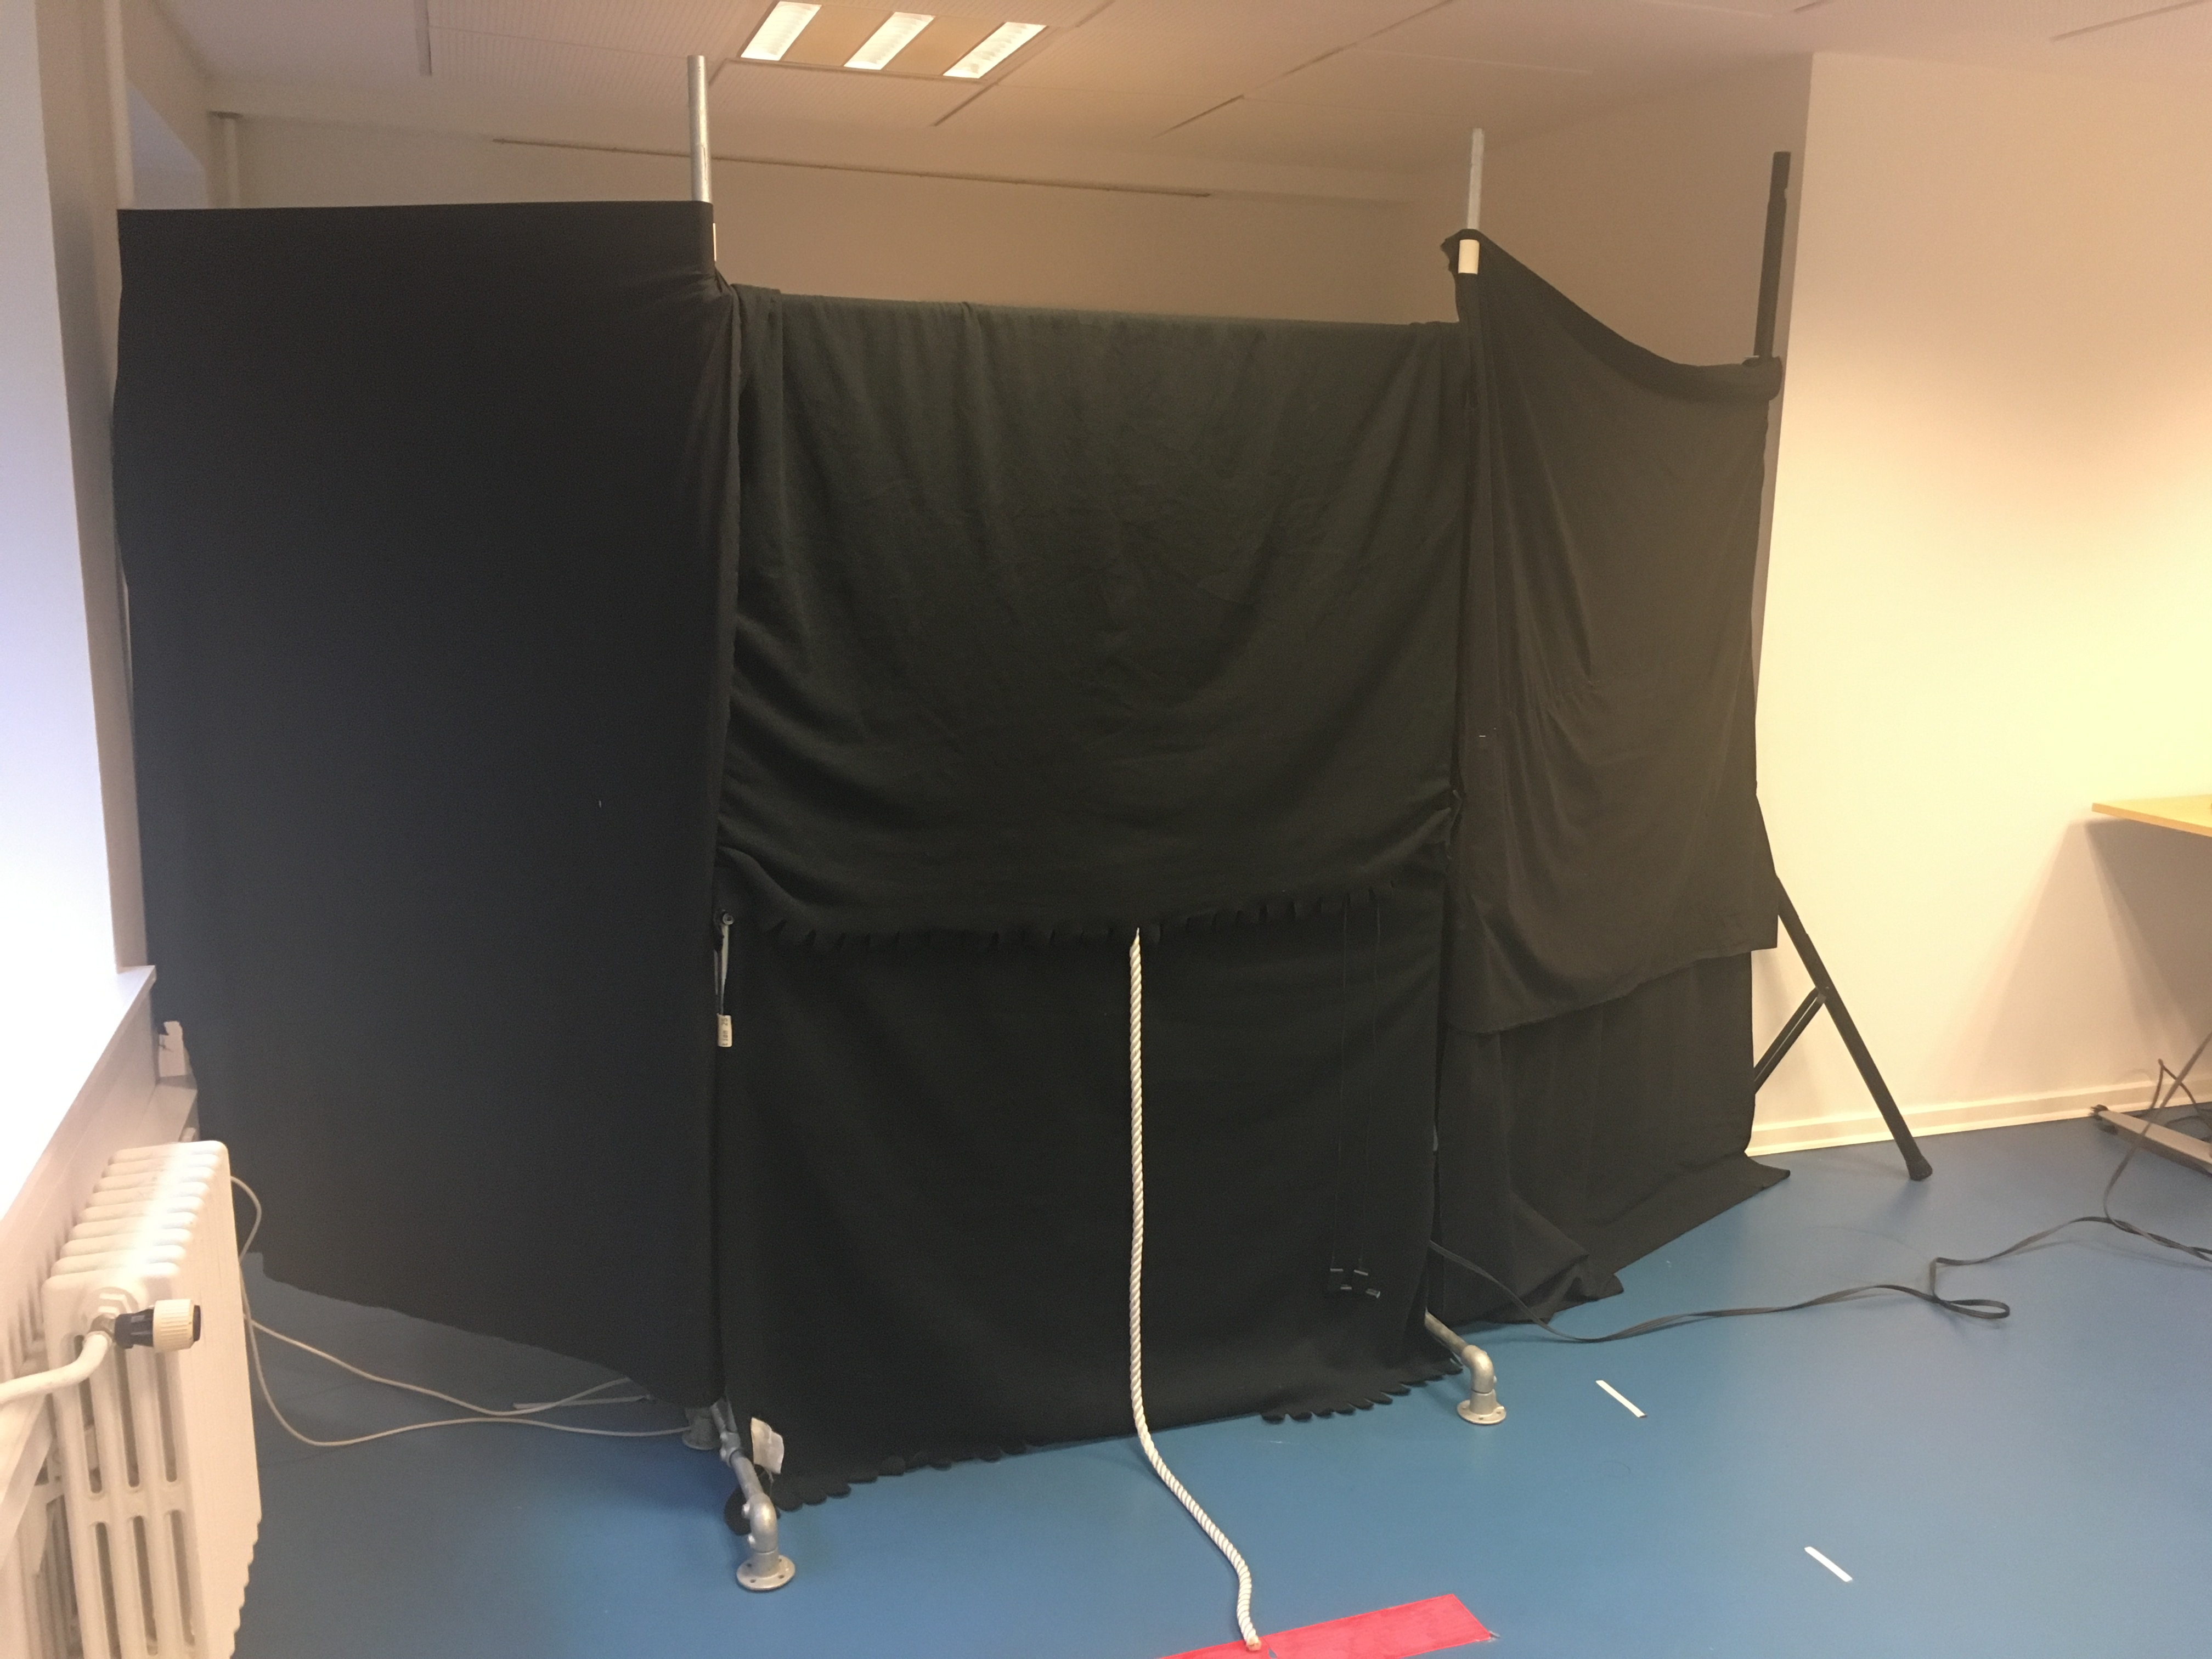
\includegraphics[width=\textwidth]{Images/setup1.JPG}
  \end{minipage}
  \hfill
  \begin{minipage}[b]{0.4\textwidth}
    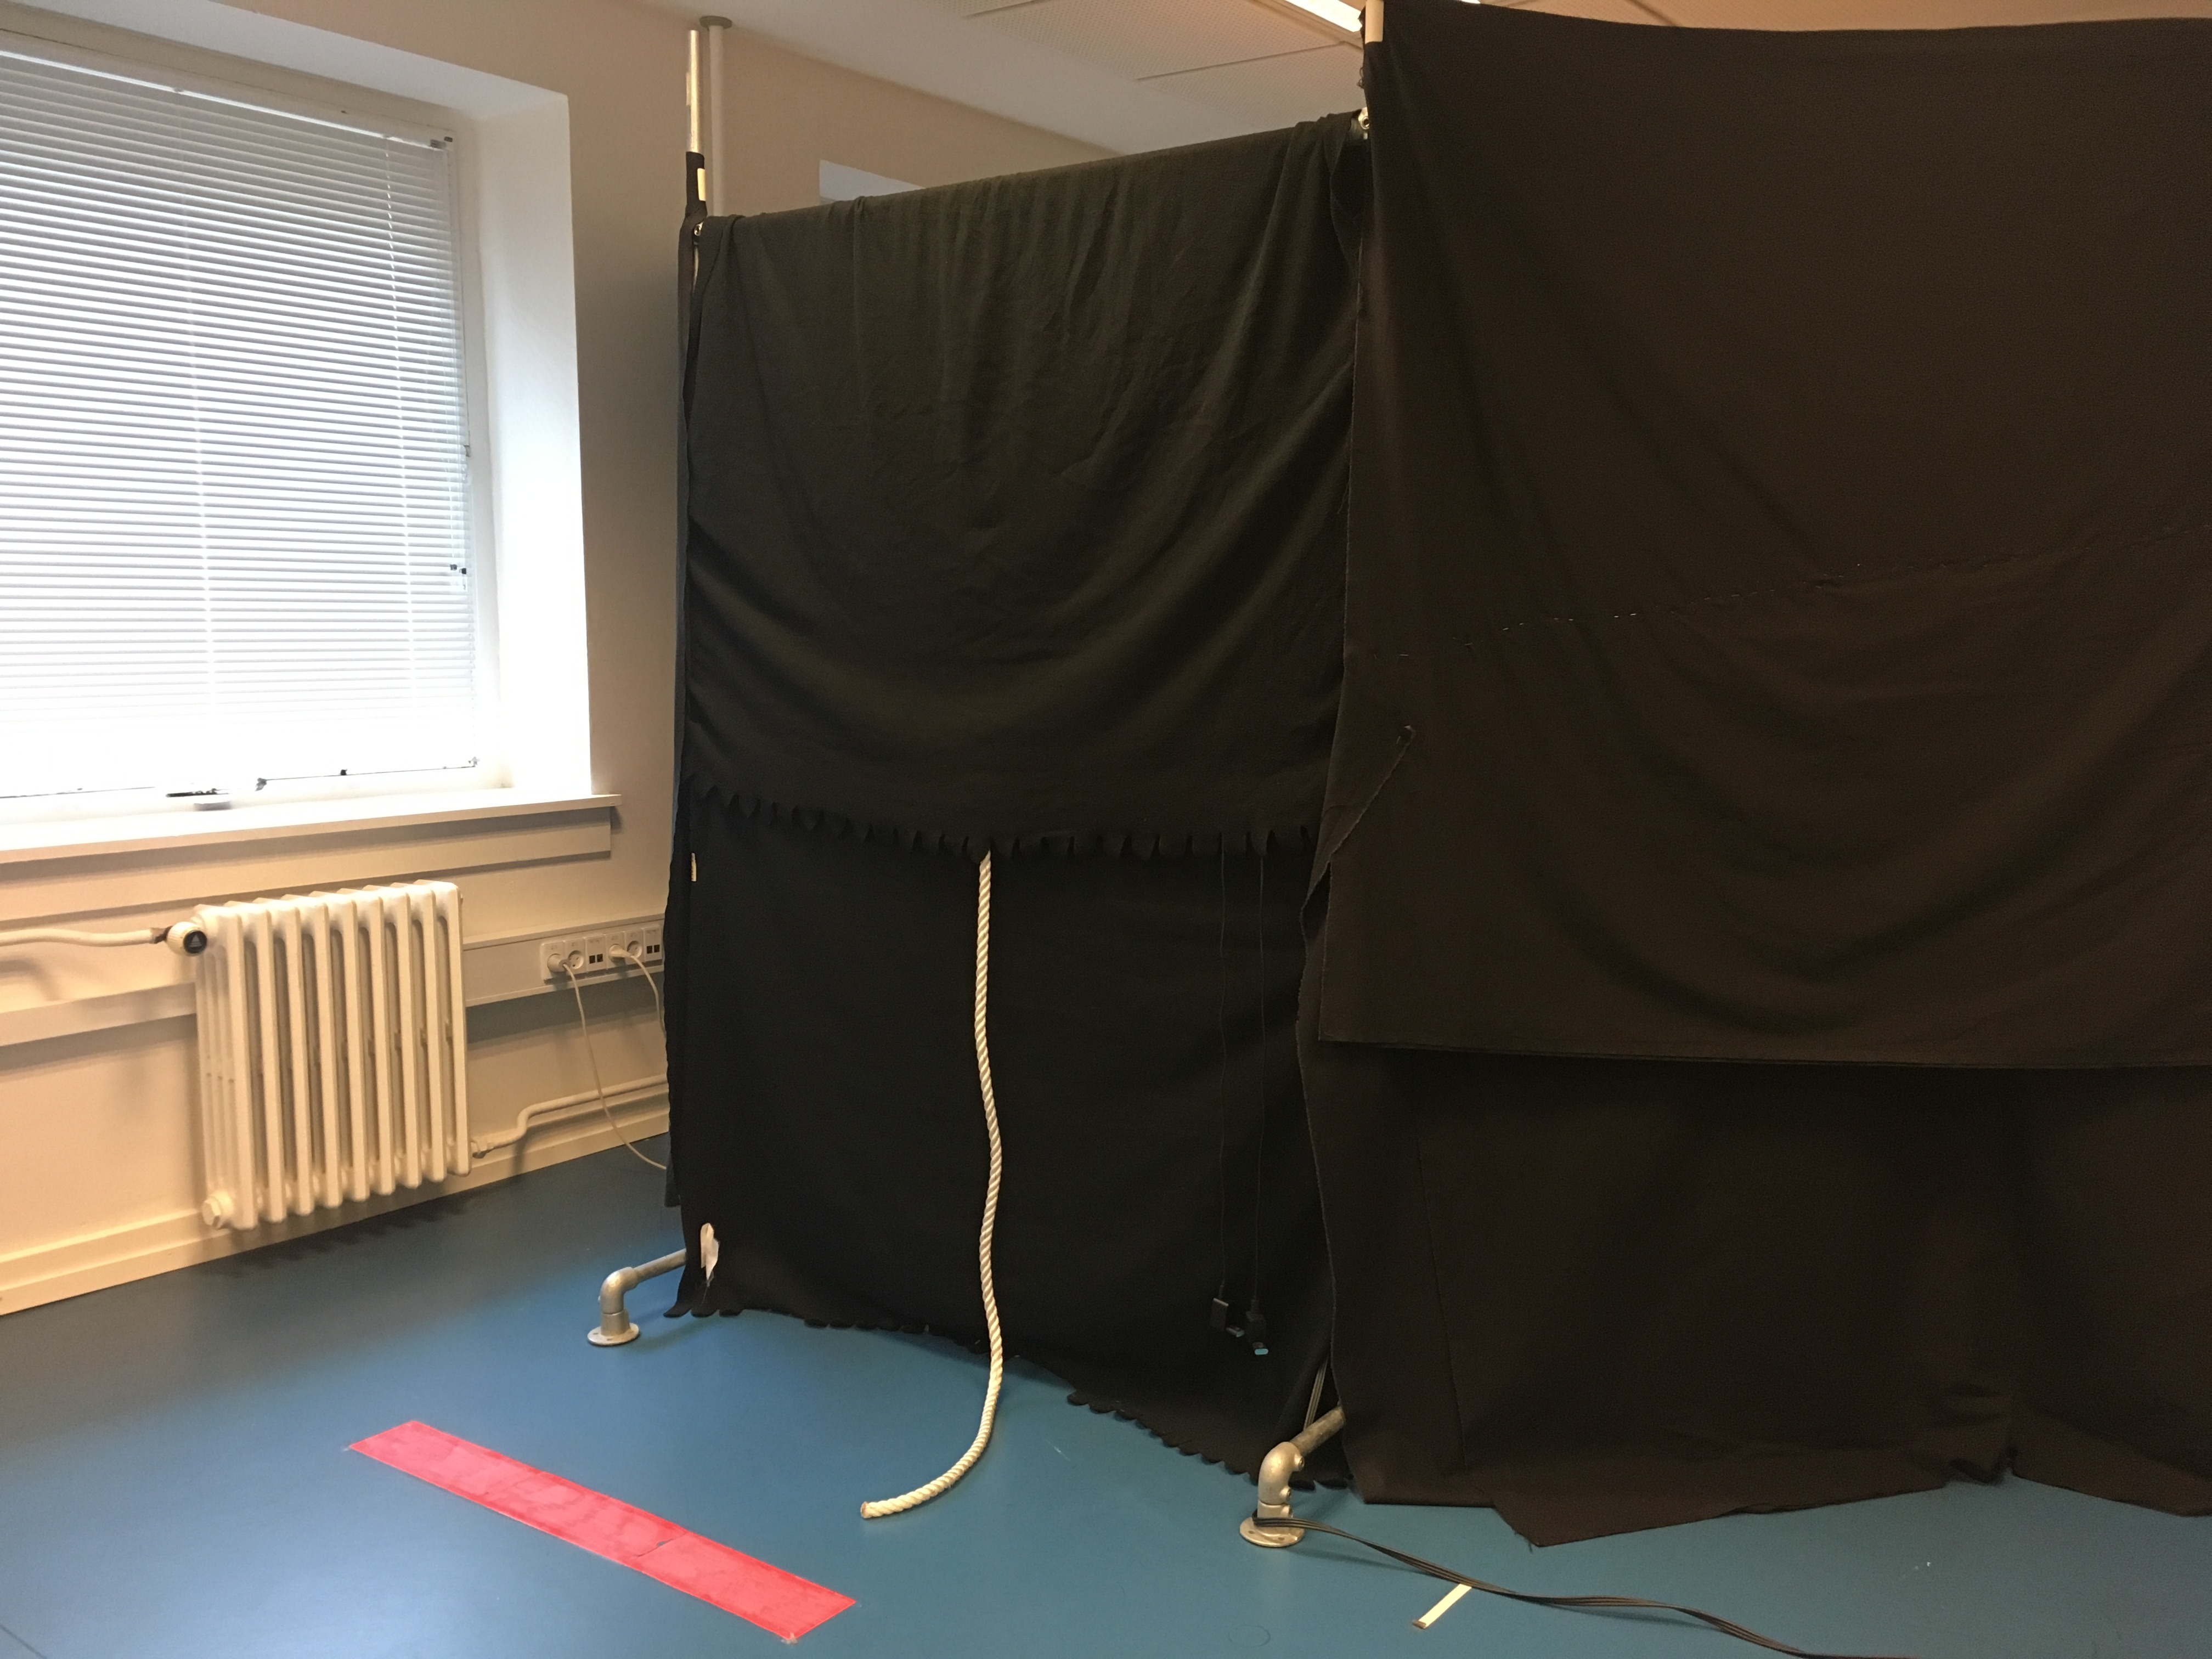
\includegraphics[width=\textwidth]{Images/setup2.JPG}
  \end{minipage}
\hspace*{\fill}
     \caption{Participants' view of the setup.}
     \label{fig:setupBlack}
\end{figure}
\begin{figure}
  \centering
  \captionsetup{justification=centering,margin=0.1cm}
\hspace*{\fill}
  \begin{minipage}[b]{0.4\textwidth}
    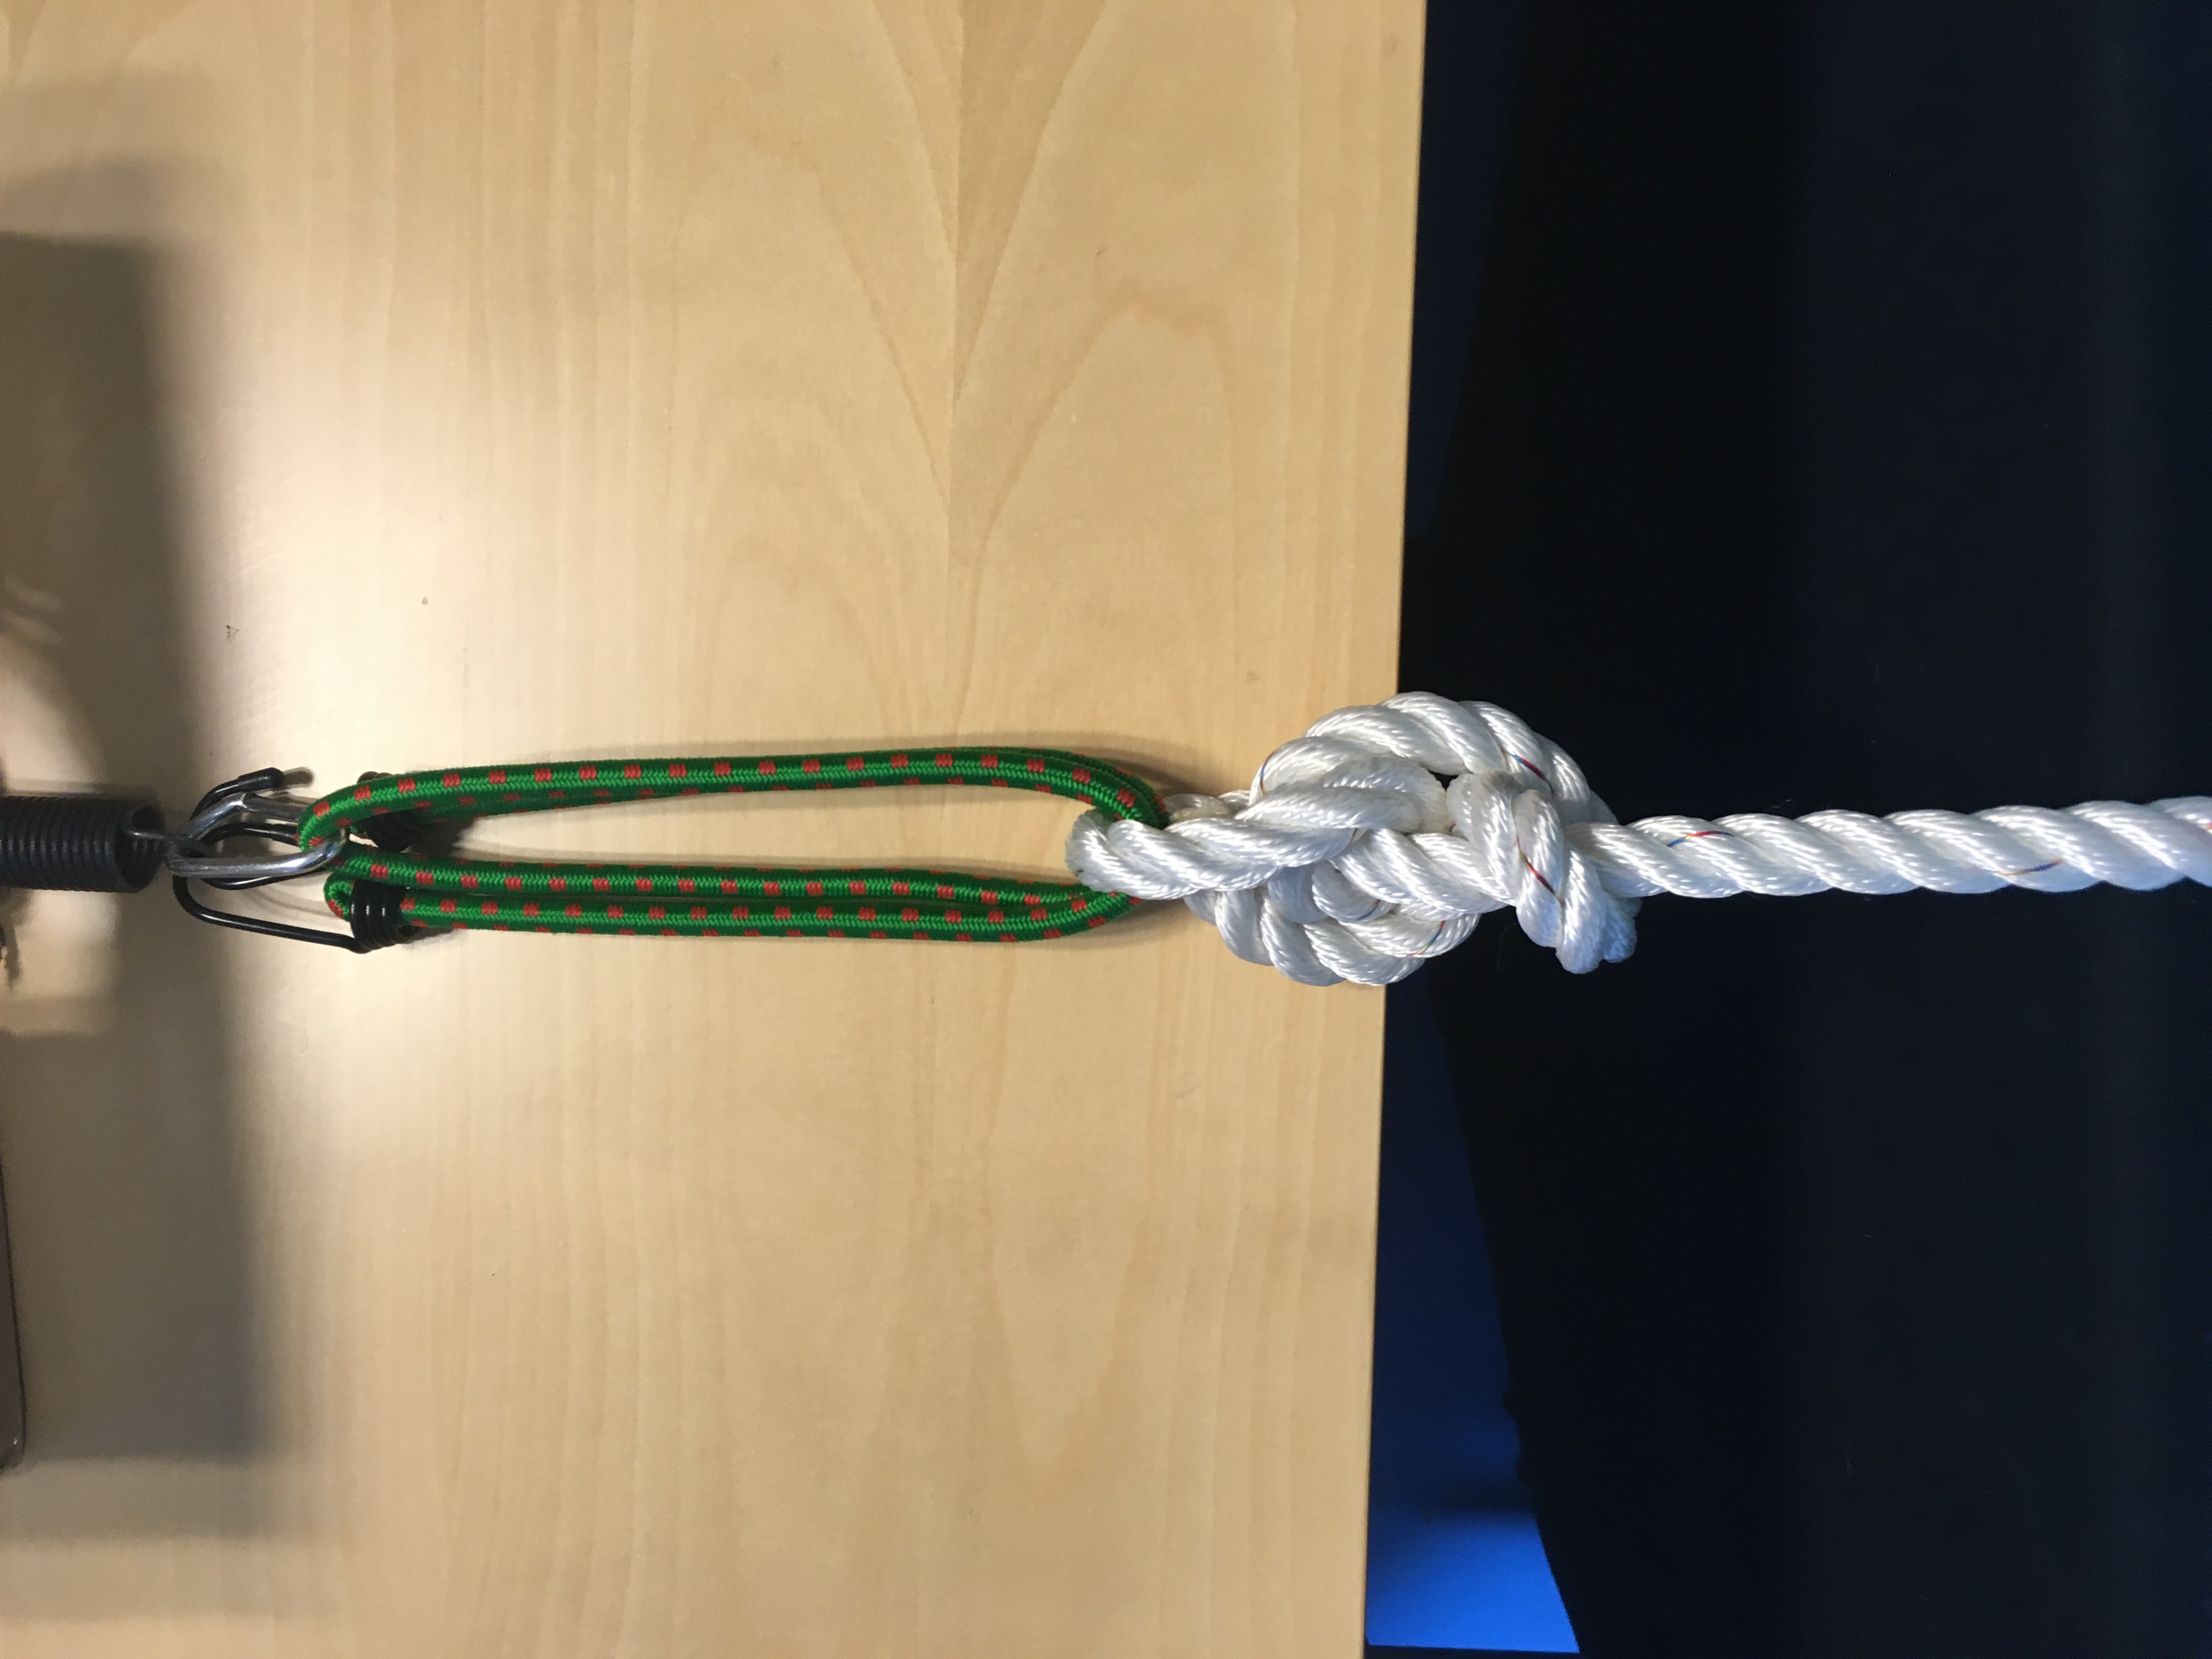
\includegraphics[width=\textwidth]{Images/rope.JPG}
    \caption{Rope and spring tied to the meter.}
     \label{fig:setupRopeBox1}
    \end{minipage}
  \hfill
  \begin{minipage}[b]{0.4\textwidth}
    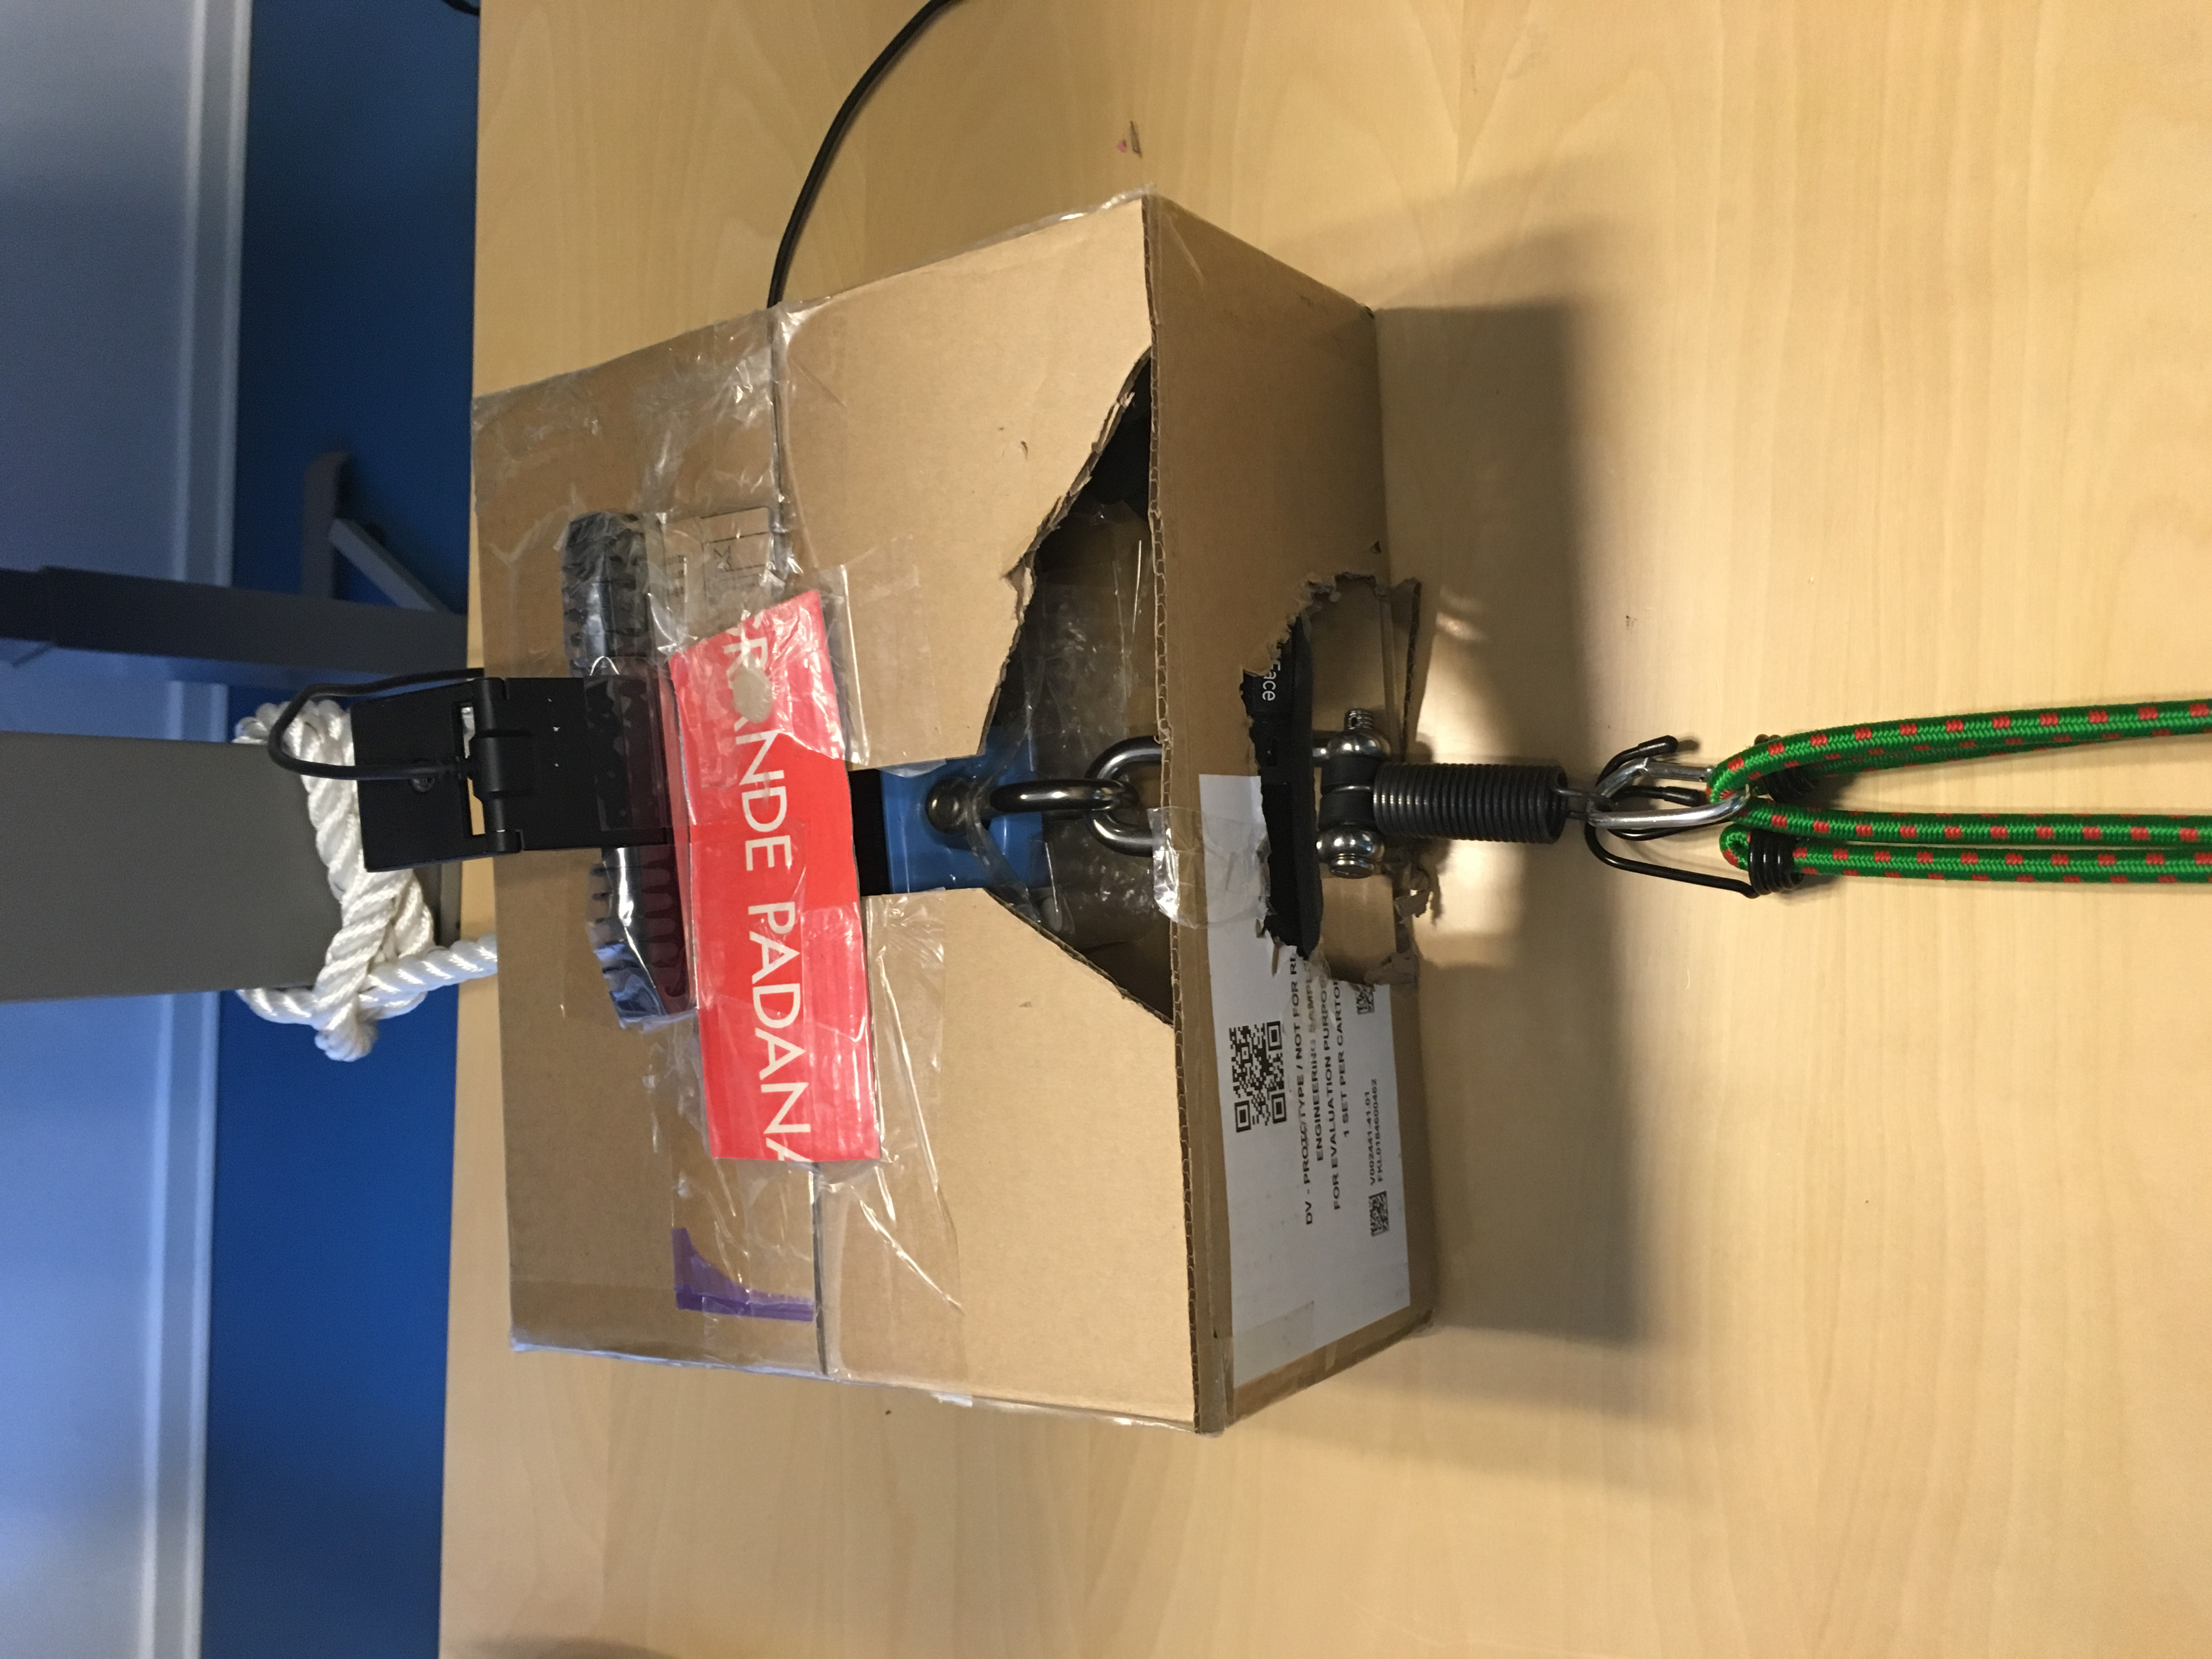
\includegraphics[width=\textwidth]{Images/BoxBig.JPG}
    \caption{Box with force meter and camera.}
     \label{fig:setupRopeBox2}
  \end{minipage}
\hspace*{\fill}
\end{figure}

\subsection{Procedure}
We greeted participants and briefly explained the broad purpose of the study. After that, we gave them two consent forms to fill in and further explained details and constraints of the tug-of-war game. Before giving participants the VR headset and gloves, they filled in a short survey with demographic data. The experimental procedure is fully explained in section \ref{subsection:instructionSheet}.
\\
Before starting the game, we calibrated the gloves for participants' hands. For each rope-pulling trial, participants were told to start pulling after the end of the countdown, when they they see \textit{Start}, and keep pulling until they see \textit{Stop}. They also received audio feedback for the countdown. Participants were told to follow two constraints: always keep their hands on the rope and try pulling the rope without moving their legs. Between rope-pulls, participants answered the questions on the quiz panel (figure \ref{fig:VRPanel}) from within the VE. After 5 rope-pulls, the game ends and participants are asked to fill in the post-experimental survey. The survey questions of the avatar appearances were gender-matched. Before participants left, we collected feedback about the game and then debriefed users about the true scope of the study.\\
For each trial, users pulled the rope for 10 seconds. Before that, they were in the VE with their opponent for 20 seconds. After the pulling ended, they remained in the same VR state for an additional 10 seconds. During this time, users could inspect the appearance of the avatars. Only after that, participants were shown the quiz panel. Transition between the game states (rope-pulling and quiz panel) was realized through a black splash screen. When the screen faded to black, the objects in the room changed. The screen fades back when the changes are complete. We did this in order to maintain a natural state of the room and prevent breaks in presence and immersion. Further details about the implementation are presented in section \ref{section:implementation}.\\
\subsection{Participants}
\label{subsection:participantsExperiment}
In order to give the appearance of a gaming study, we designed a poster to recruit people for the experiment. We placed this poster (\ref{subsection:poster}) around the university campus and  used it for recruiting messages. For the user study, we recruited a total of 28 participants (17 female) from the university campus and local Facebook groups. They were between 21 and 34 years old $(M = 24.42, SD = 3.06)$. Participants were unable to take part in the study if they previously completed the avatar appearance survey. We discarded the results of 2 participants (1 female) due to invalid data. Of the remaining ones, 9 participants had never used VR before and 16 had never played real-life tug-of-war. Participants were rewarded with a gift valued at 100 danish krone for taking part in the whole study.

\begin{figure}[H]
  \centering
  \captionsetup{justification=centering,margin=0.1cm}
\hspace*{\fill}
  \begin{minipage}[b]{0.4\textwidth}
    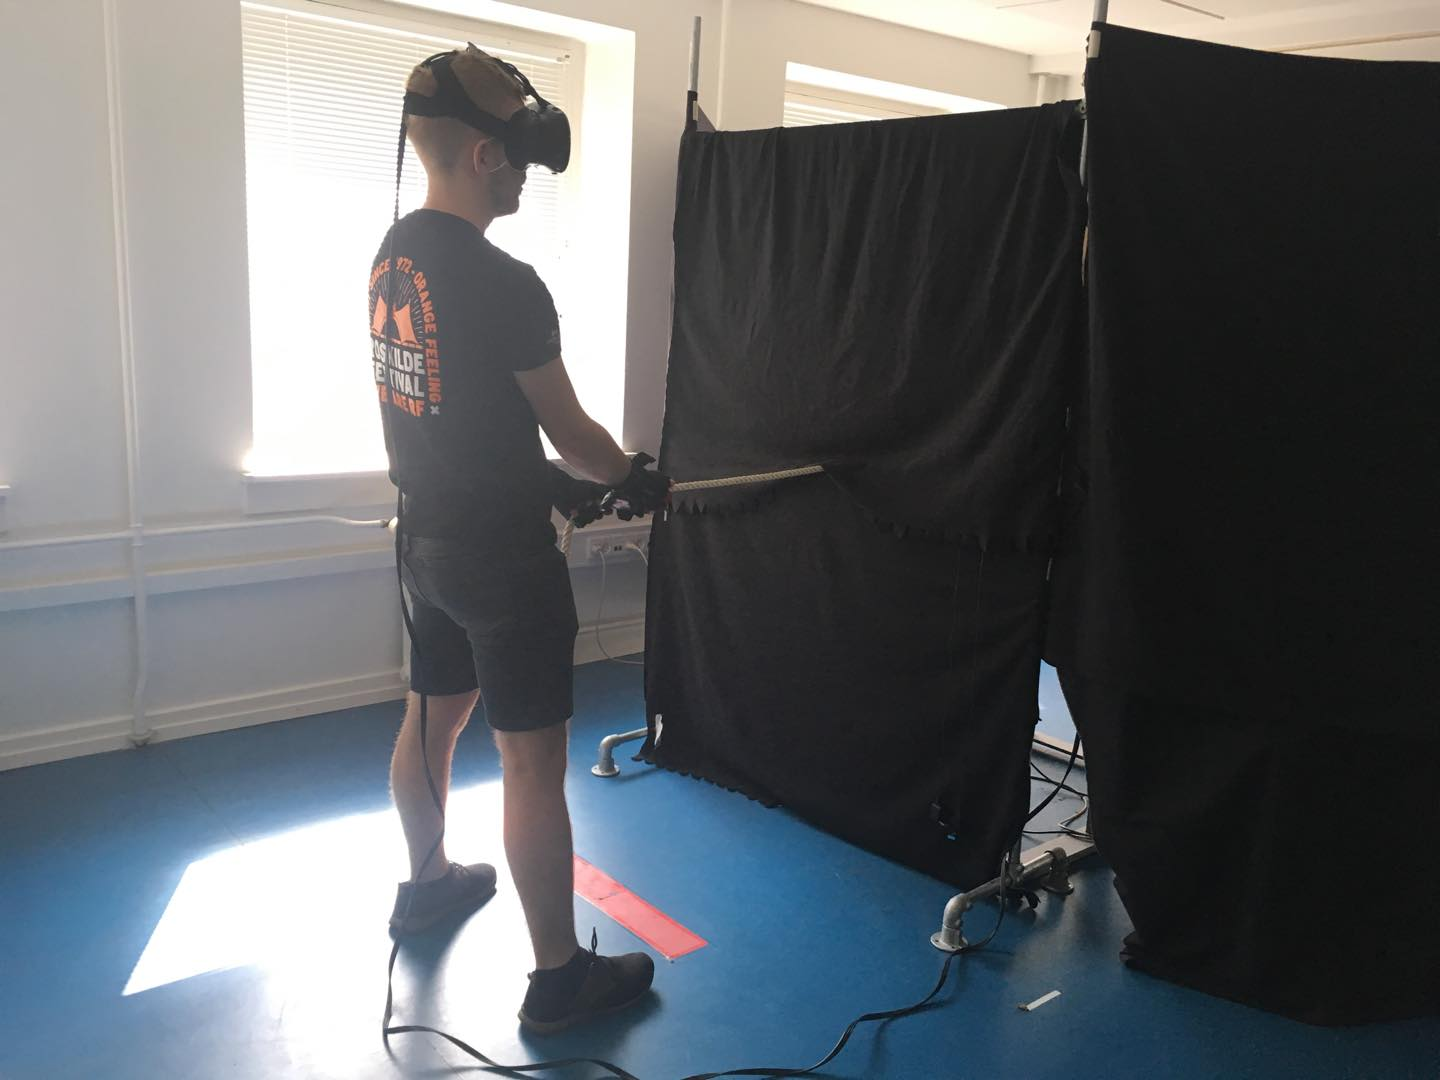
\includegraphics[width=\textwidth]{Images/Participants/m1.jpg}
  \end{minipage}
  \hfill
  \begin{minipage}[b]{0.4\textwidth}
    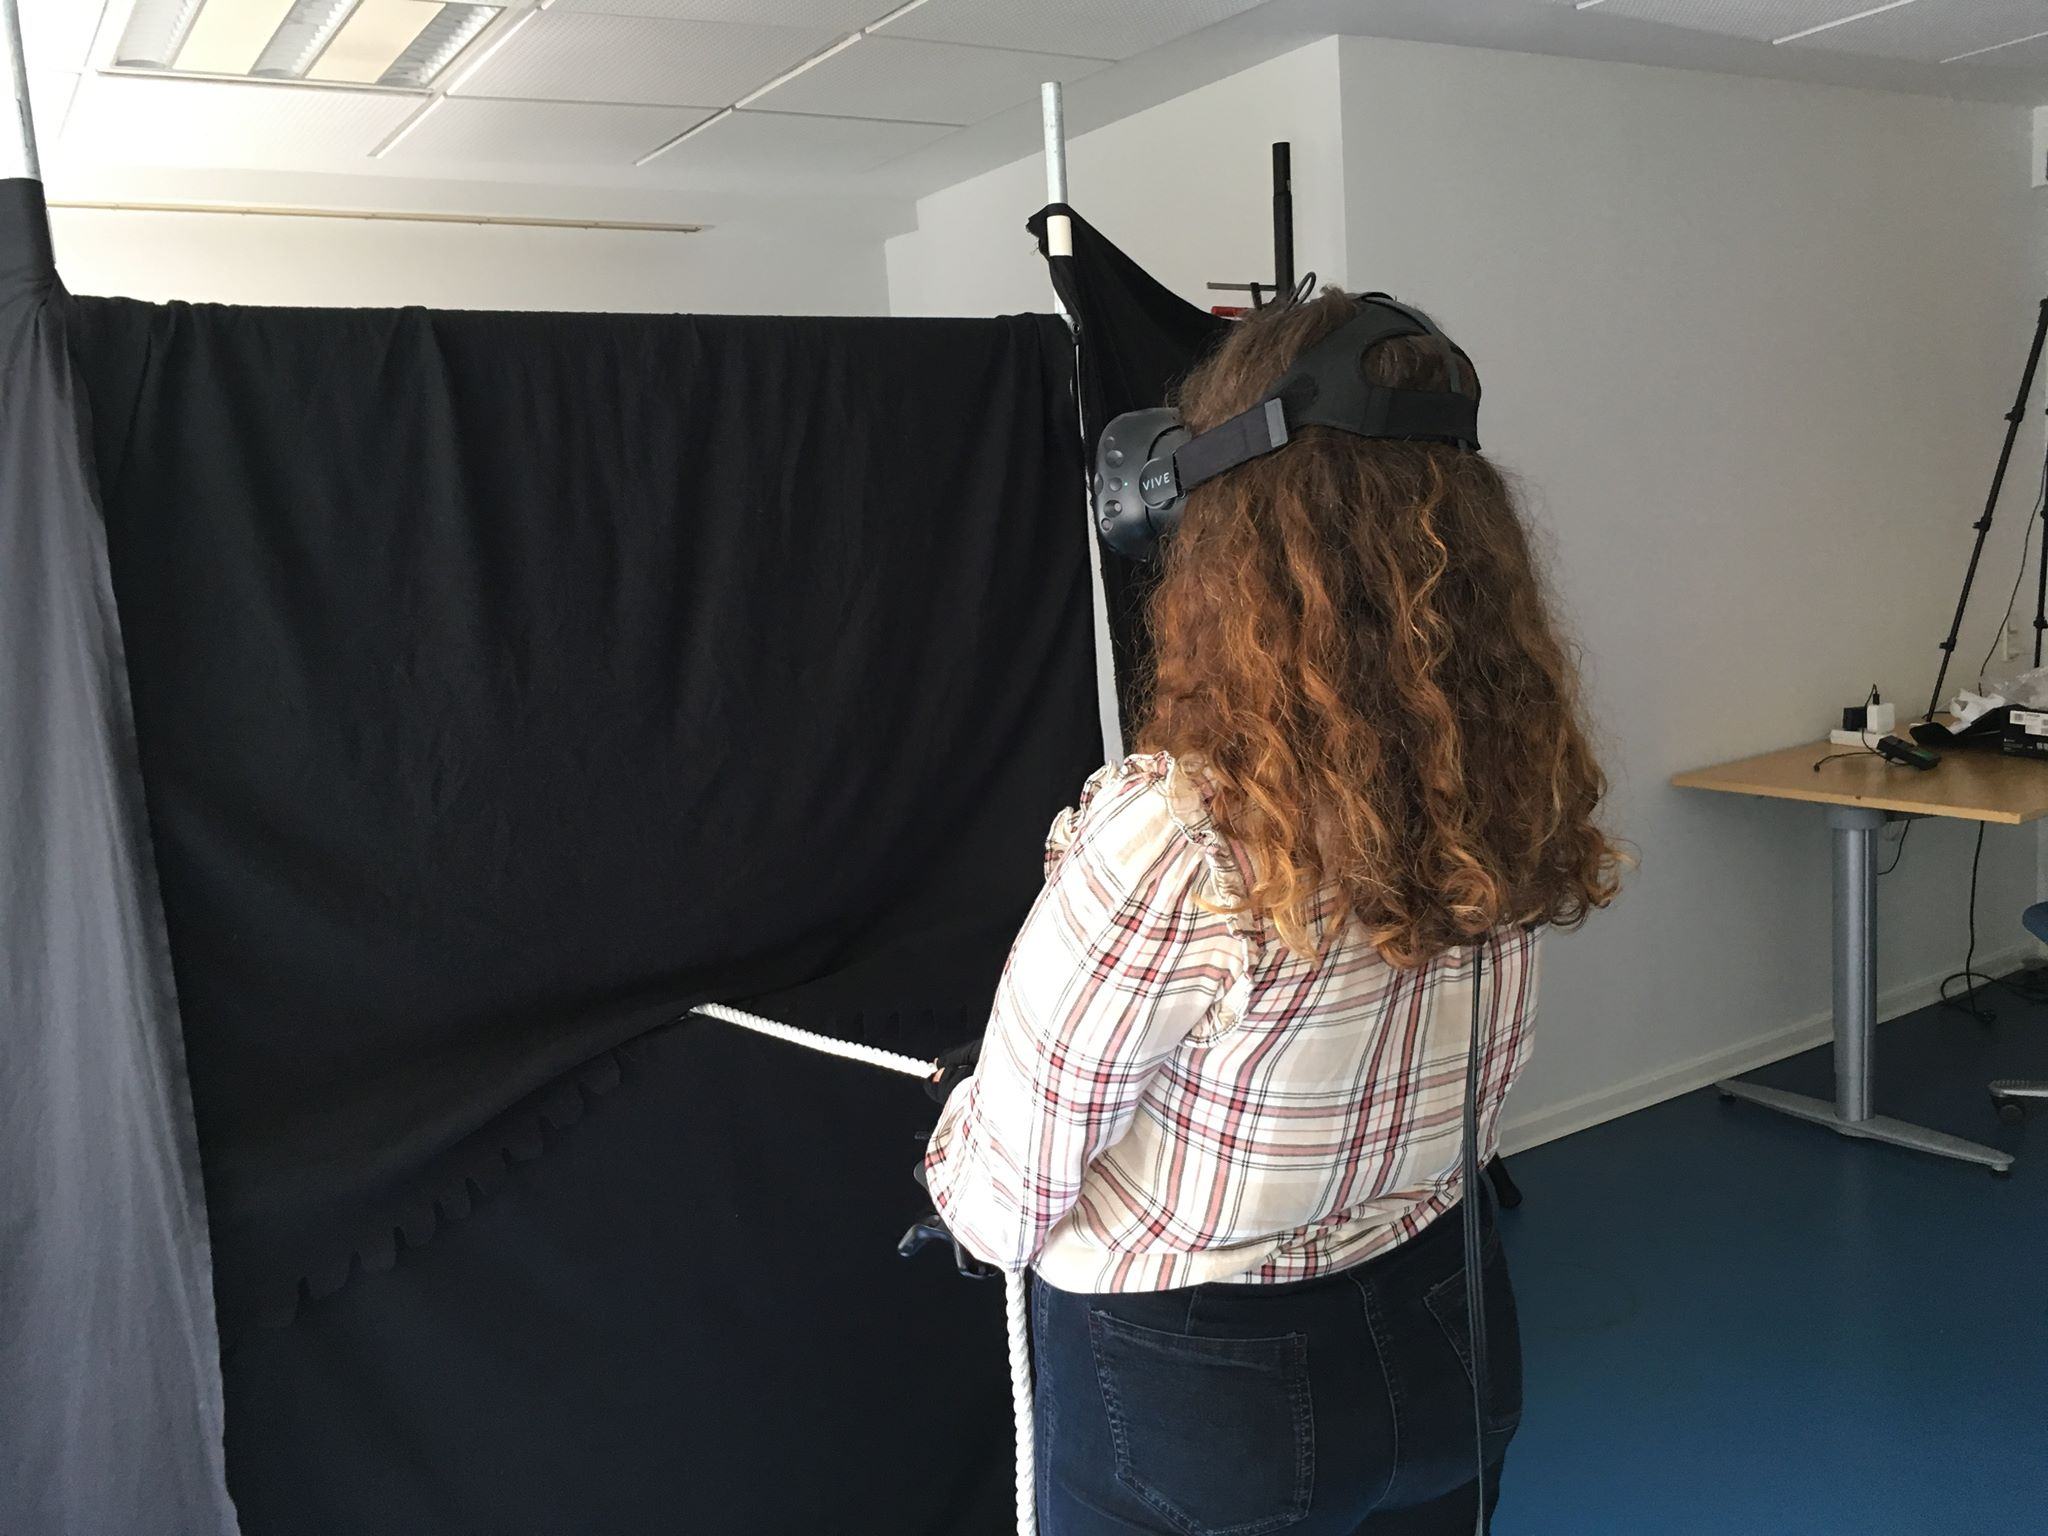
\includegraphics[width=\textwidth]{Images/Participants/f1.jpg}
  \end{minipage}
\hspace*{\fill}
     \caption{Participants playing tug-of-war VR  .}
     \label{fig:participants}
\end{figure}
\subsection{Results and Discussion}
The results were manually logged by the experimenter. To measure the maximum force, we looked at the force meter data from the end of the countdown, at the beginning of the \textit{Start} message, until the end of the \textit{Stop} message. All force data presented is measured in kilograms. In the plots below, we present data in terms of ordering and condition. By ordering, we mean the order in which participants saw the appearances, labeled as \textit{Trial}. By condition we mean the condition of the opponent participants faced, labeled as \textit{Condition}. Trial 1 refers to the first trial of rope-pulling participants performed, out of a total of five. Trial 2 refers to the second one and so on. The condition captures the independent variable and represents a numerical mapping from 1 to 5 to the appearance variable, increasing by strength/intimidation. Condition 1 refers to the weakest-looking chosen avatars according to the weighted score (see \ref{fig:SurveyRatedFemalesChosen},\ref{fig:SurveyRatedMalesChosen}) and condition 5 refers to the strongest looking avatars. We also display our results by gender. \\
Considering the large amount of information presented, we structure the results section as follows:
\begin{enumerate}
\itemsep0.1em
    \item For each subsection we start with a short paragraph describing the main findings, if applicable;
    \item We give an overview of the results;
    \item We discuss the results with respect to related work and speculate on our respective findings;
    \item At the end, we present a summary of all our findings and discuss implications.
\end{enumerate}

\subsubsection{Conditions per Trial}
\begin{figure}[H]
\vspace*{-3mm}
 \centering
 \captionsetup{justification=centering,margin=0.1cm}
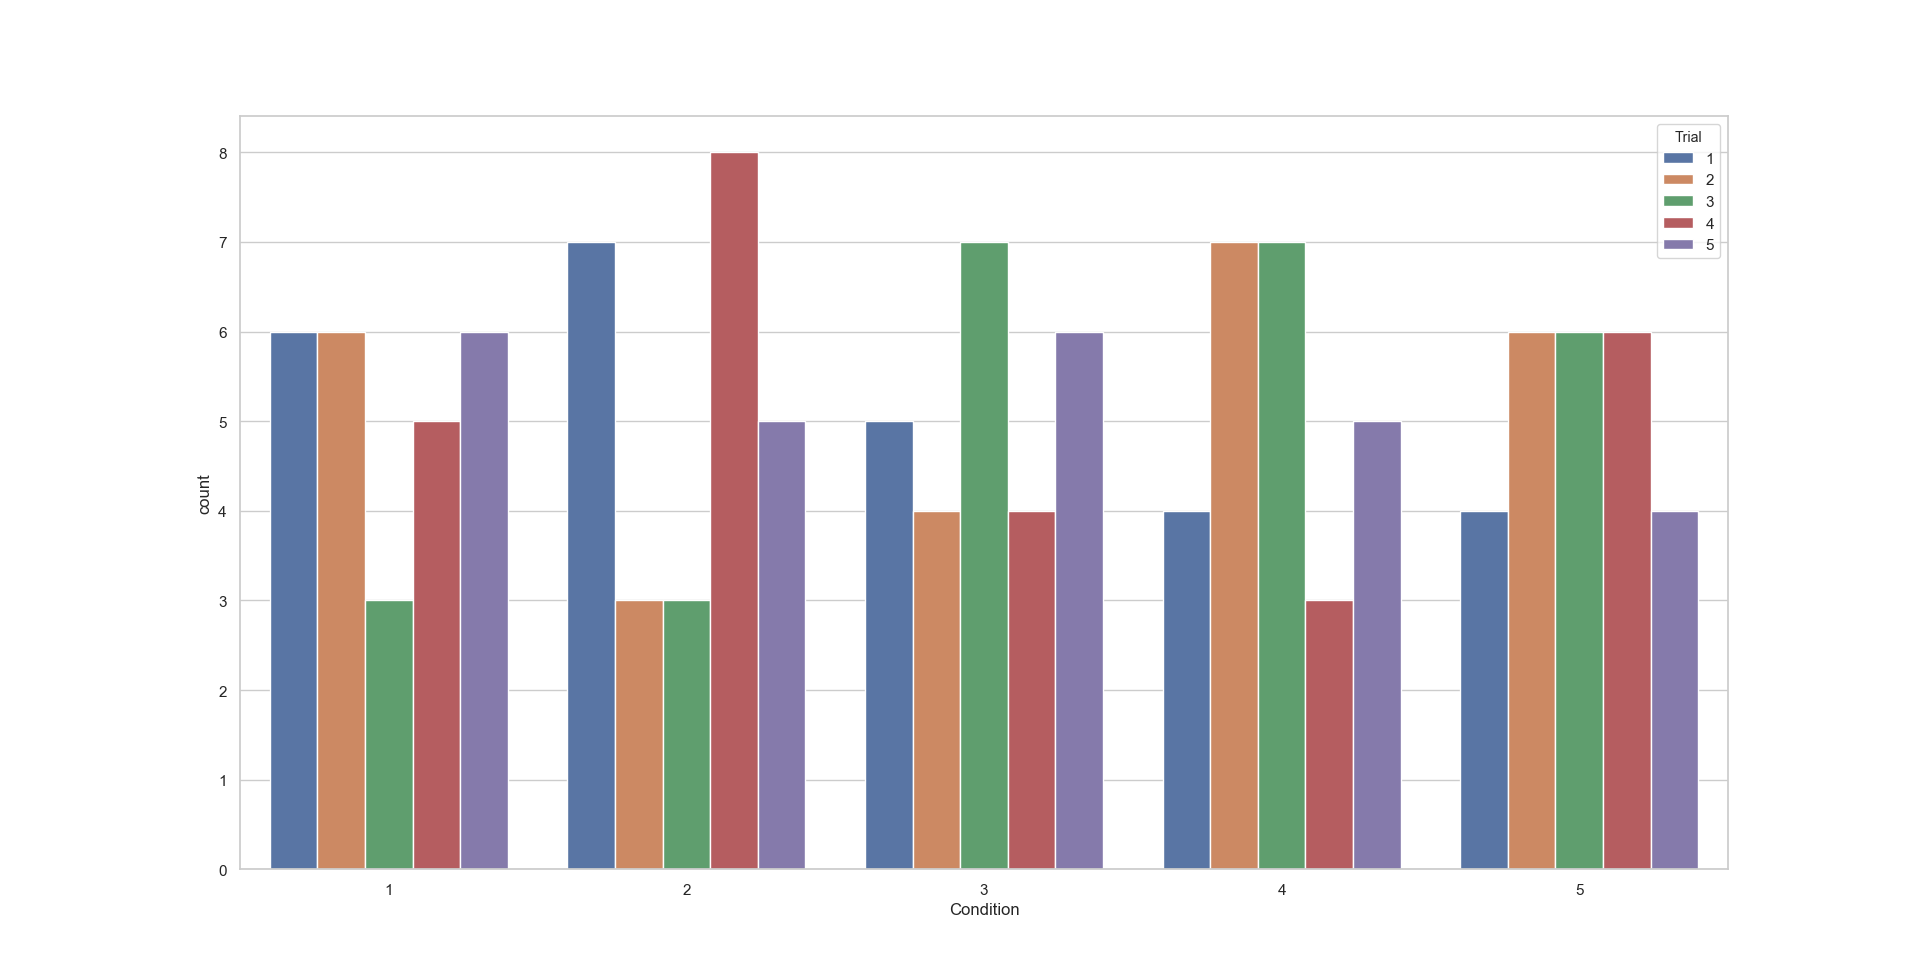
\includegraphics[width=0.9\textwidth]{Files/Plots/condition_by_trial.png}
 \caption{Number of conditions per trial.}
 \label{fig:condPerTrial}
  \end{figure}

In the above pictures we show the distribution of each condition for each trial. Since the conditions were randomized, there may be an effect of over-representation. The fifth trial seems to be the most balanced, representation wise.
We had more female participants and thus more female avatars were evaluated. For an overview of the distribution of conditions per trial for males and females please section \ref{subsection:additionalData} figures \ref{fig:condPerTrialM} and \ref{fig:condPerTrialF}.

\subsubsection{Appearance Ratings}
\begin{figure}[H]
 \hspace*{\fill}
     \begin{subfigure}[b]{0.4\textwidth}
         \centering
         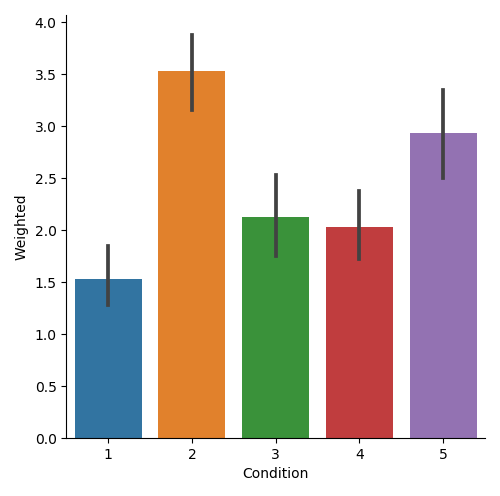
\includegraphics[width=\textwidth]{Files/Plots/weighted_ratings_female_experiment.png}
         \caption{Ratings for female avatars.}
         \label{fig:weightedFEx}
     \end{subfigure}
      \hspace*{\fill}
     \begin{subfigure}[b]{0.4\textwidth}
         \centering
         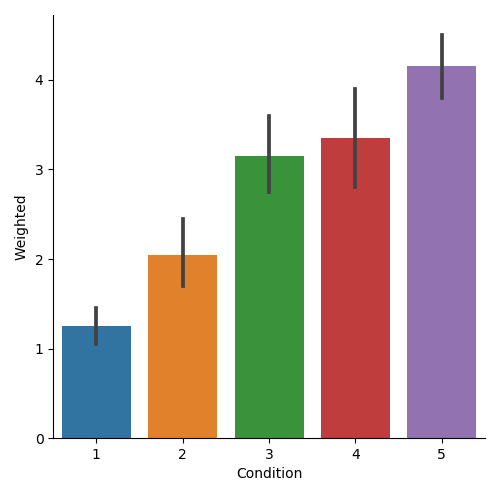
\includegraphics[width=\textwidth]{Files/Plots/weighted_ratings_male_experiment.png}
         \caption{Ratings for male avatars.}
         \label{fig:weightedMEx}
     \end{subfigure}
      \hspace*{\fill}
     \caption{Weighted ratings by condition for the opponent avatars in the user study. Error bars show 95\%  confidence interval.}
         \label{fig:weightedEX}
\end{figure} 
\textbf{Results}  \\
Participants rated the appearance of same-gender avatars on attractiveness, intimidation, intelligence and strength. In the above  figures we present the weighed results of those ratings for female (\ref{fig:weightedFEx}) and male (\ref{fig:weightedMEx}) avatars. The weighted value is computed as: $weighted=0.5strength+0.5intimidation$.
Male participants rated the avatars as expected, increasing in intimidation and strength by condition. For females, the avatar in condition 2 (low-average) was rated as highest in intimidation and strength, while the avatar in condition 5 (strong) came second. All ratings for these avatars and their thumbnails can be found in section \ref{subsection:thumbnailsExperiment}. \\
\\
\textbf{Discussion}\\
The ratings for female avatars for the VR tug-of-war game were inconsistent with our results from the survey. There were several limitations when designing the female agents (detailed in section \ref{section:AgentDesign}) which lead to females being perceived overall as less strong and intimidating, even in the survey. One difference between the 2 studies is that participants playing tug-of-war could see the full body of the avatar in VR. On the other hand, participants filling in the survey only saw their thumbnails. Furthermore, due to the resolution of the headset, participants in VR saw the avatars with less clarity and texturing. One participant mentioned that she would have liked to see females having more hair. This aesthetic preference appears to have put off participants instead of making strength cues more salient.\

\subsubsection{Qualitative Feedback}
\label{qualitativeFeedback}
Our observations and qualitative feedback show that people experienced various degrees of physical illusions. Participants initial comments suggest that the illusions were stronger in the first few trials. As the game went on, they seemed to become aware that there is no force acting on the rope. Realism was often quoted as a reason for the breaks in illusion. With respect to this, participants suggested improving the animations and making their opponents react to their pull. The virtual rope was seen as highly realistic and holding the rope seemed to contribute to this belief.\\
\\
\textbf{Results}\\
 In total, 4 participants showed high awareness of the purpose of the experiment (``how people react when they see different people in front of them''--- P22). Among them, a few made comments about their own behavior, which seemed to support our research question (``for the people that looked stronger I had to pull more''--- P2). \\
Participants generally seemed to have an expectancy that the stronger the avatar looks, the more they should pull (``if you expect a stronger person you will pull stronger''---P14). P16 mentions `` I felt like the body shape was according to how to pull. [I was] pulling more strong for someone bigger and less for someone smaller''. In the case of P26, they, mention intimidation: ``I was expecting I would feel the need to pull harder because the characters were more intimidating from their look''.\\
With respect to the challenges, some participants clearly state feeling a distinction: ``[for one avatar] felt like it was easier''---P19, ``felt actually pulling like there was another person on the other side''---P16. Furthermore, our qualitative feedback suggests the illusions were breaking as trials went on. In the case of P13, her feedback in the first trial was that: ``It's weird - I can feel something pulling''. Eventually, in the post-experimental interview she mentions that ``sometimes they were pulling without me feeling''. P4 remarks: ``the machine did not make much effort pulling back'' and that ``[it] was not consistent with the guys [referring to opponents]''. However, in the end they state:``[it] lost realism when I realized it isn't pulling back''. P15 remarks feeling a difference in the first trials, but not in the last ones --- ``didn't see a difference in challenge in the last 2 ones''. P9 comments: ``I can tell the difference between the challenges''. However, by the end they conclude referring to the opponents that it ``didn't feel like they were pulling''. One participants adds that the appearances made him think about his own abilities: ``I think it was the same strength but, in a way, since you are not prepared for that, maybe you feel weak'' (P18).\\
Some participants were unsure if they had felt any difference and used ambiguous language to suggest they felt little to no variation: ``can't tell if there was a difference or not in pulling''---P15, ``more or less the same strength''---P24, ``did not feel that much of a difference in enemies''---P28. P8 then adds that it seemed like they were ``receiving same amount as putting into it''. They admit feeling ``resistance'', however it was ``difficult to tell''. Acknowledging some perception incongruities, P25 says that: ``I wasn't sure if I should feel the pressure, but I could see them pulling so you created that impression a bit''.\\
Others mentioned not feeling any difference throughout the experiment: ``didn't feel physical challenge of a counterattack''~(P17), ``feels like it's the same challenge'' (P12). Often, participants referred to lack of realism when pointing out downsides of the game: ``when I was trying to pull harder, [I] didn't have my body being pulled''---P17. They were mostly disappointed that their opponents were not reacting properly to their pull: ~``always leaned back no matter how much I pulled''--P23, ``if you pull harder you expect them to come closer, lose balance or pull harder''---P14.  They suggested ``make[ing] the other avatar move or fall'' (P7) or adding sounds: ``avatars made it look more unreal, it looked silent; make them talk with some sounds'' (P16). When their expectations about the game were not met, the realism of the experience decreases (``didn't feel real because they were not pulling stronger when they looked stronger''---P9). Some participants noticed that the avatars were animated in the same way, which also had an impact: ``avatars doing the same, kind of the same move, doesn't feel realistic''---P11. Additionally, users desired their opponents to be more \textit{expressive} (P27). Beyond avatar design, a participant mentions that ``being able to also move your feet would be good'' (P11). One participant disliked that the textures and shading in the game were not detailed enough (P6). In their opinion, these design enhancements were required to generate a realistic setting. \\
In contrast, there were some participants who found the experience highly realistic ``Felt real like really against an opponent'' (P1). The rope was often mentioned as a good source of realism for the game:``Felt more real because I was holding something''--P9. The haptic feedback seemed to made the virtual rope even more real, one participant mentioning: ``I didn't look as much at my hands as I thought [...] I could feel the rope ''. P16 remarks: ``I played VR before, but never like pulling an object and seeing it in VR [...] It helps that you feel the rope and see the rope''.
Few mentioned any downsides of the rope (``rope was too elastic''---P15).\\
Participants did not generally make comments about their arms. Some noticed inaccuracies in their avatars: ``Arms seemed off when I looked straight at them''---P4. For example, P1 had a highly realistic experience (``I really had a feeling like I was in that room'') , but mentions the arms \textit{twisted around}, and ''everything else felt more responsive than the arms''. //
We also noted that sometimes participants dynamically changed their standards for the challenge ratings: ``I'm getting tired more so I will give it a 5''---P11. P10 mentions that he begins to give 5 challenge ratings because of lack of feedback:``I feel like I'm not making any progress; they are not moving at all ''.\\
\\
\textbf{Discussion}\\
Overall, from their feedback and our observations, participants seemed to use the system in unexpected ways. Their comments 
suggest that they tested the way in which opponents pulled. In one example, P23 acknowledges straying from experimenter instructions to test their assumption. After the game, P23 mentions that when they saw a \textit{strong guy} they \textit{expected} them to pull harder, so they pulled less to feel it. When logging the results of the force meter and during the game we also noticed participants were pulling the rope in various ways. They were instructed to pull the rope and keep pulling until they see \textit{Stop}, however many  users tugged at the rope, pushed it back and forth instead of keeping it at maximum exertion.\\
Moreover, other participants  seemed to be affected by the novelty of the experience. P10 was surprised that they actually had to pull the rope and realized this only after the trial began, when the experimenter remarked they should pull the rope. The first trial had other design problems. Three participants used their legs initially and pulled too hard, moving the equipment. They realized they could not pull so hard and restricted themselves in the following trials. Other participants also displayed this restraining behavior and reluctance to pull hard.
\subsubsection{Force Meter Data (H2)}
\begin{figure}[H]
\hspace*{\fill}
     \begin{subfigure}[b]{0.4\textwidth}
         \centering
         \vspace*{-10mm}
         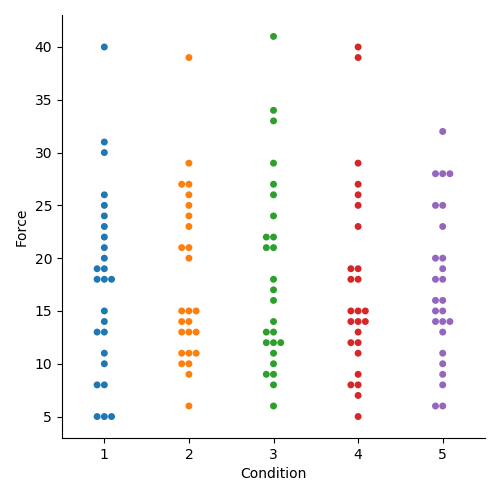
\includegraphics[width=\textwidth]{Files/Plots/force_by_cond_swarm.png}
         \caption{All force values by condition.}
         \label{fig:allForceSwarm}
     \end{subfigure}
     \hspace*{\fill}
     \begin{subfigure}[b]{0.4\textwidth}
         \centering
         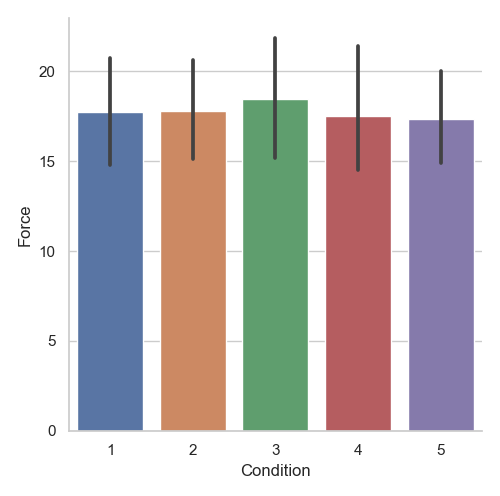
\includegraphics[width=\textwidth]{Files/Plots/force_mean_by_condition.png}
         \caption{Mean force by condition}
         \label{fig:allForceMeanCond}
     \end{subfigure}          
     \hspace*{\fill}
     \begin{subfigure}[b]{0.4\textwidth}
         \centering
         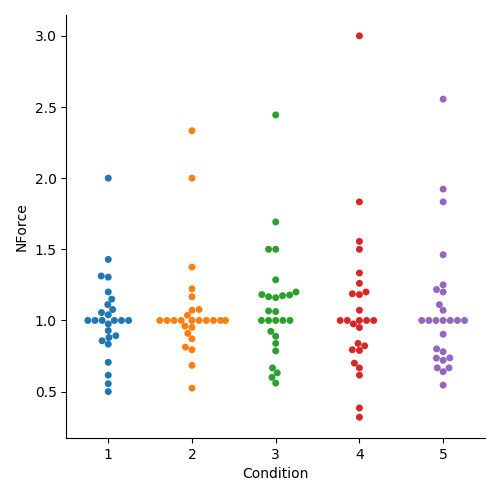
\includegraphics[width=\textwidth]{Files/Plots/forceNforce_by_cond_swarm.png}
         \caption{All N1 by condition. }
         \label{fig:allN1NCond}
     \end{subfigure}
     \hspace*{\fill}
     \begin{subfigure}[b]{0.4\textwidth}
         \centering
         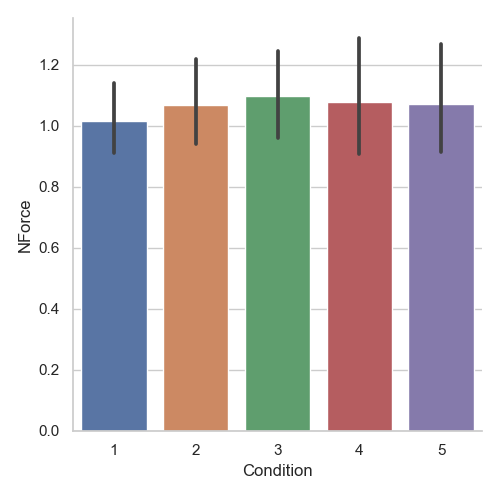
\includegraphics[width=\textwidth]{Files/Plots/forceNforce_mean_by_condition.png}
         \caption{Mean of N1  by condition. }
         \label{fig:meanN1Cond}
     \end{subfigure} 
     \hspace*{\fill}
         \begin{subfigure}[b]{0.4\textwidth}
         \centering
         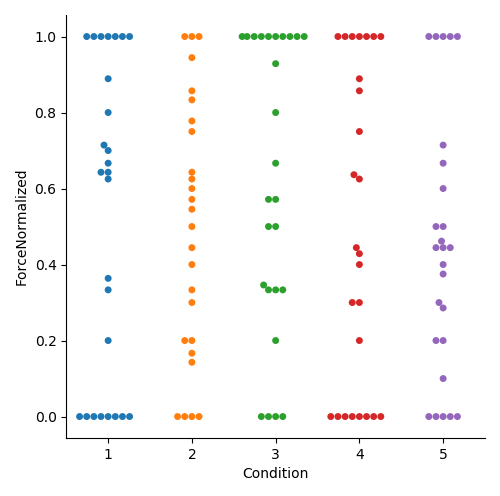
\includegraphics[width=\textwidth]{Files/Plots/forceNormalized_by_cond_swarm.png}
         \caption{All N2 by condition.}
         \label{fig:allN2Norm}
     \end{subfigure}
\hspace*{\fill}
     \begin{subfigure}[b]{0.4\textwidth}
         \centering
         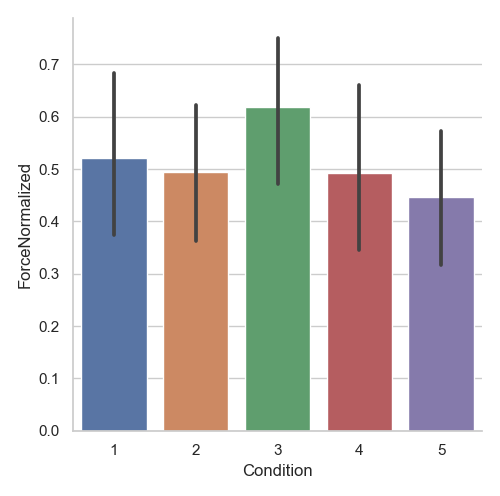
\includegraphics[width=\textwidth]{Files/Plots/forceNormalized_mean_by_condition.png}
         \caption{Mean of N2 by condition.}
         \label{fig:meanN2Cond}
     \end{subfigure} 
      \caption{All force (kg) values by condition. Error bars show 95\%  confidence interval.}
         \label{fig:allForceCond}
\end{figure} 
 Despite positive qualitative feedback, there were inconsistencies in how strong participants pulled. We expected some variability because users interacted with the system in unforeseen ways. These quantitative results, however, do not appear to support H2.\\
 \\
\textbf{Results}\\
In the above figures we show an overview of all the data measured from the force meter, namely the maximum force pulled for each trial (kg). We normalize this data in two ways, N1 and N2. In the case of N1, for each participant we subtract from all trials the value in the first trial. For N2, we normalize values between 0 and 1 with min-max normalization. We take the minimum and maximum for each participant from all their respective trials. The normalization formulas are as follows: 
\[ N1_i^p=X_i^p-X_1^p, i \in \{1,2,3,4,5\},\; i \; trial \; number,\; p \in PIDS \]
\[N1= \{ N1_i^p |  i \in \{1,2,3,4,5\},\; i \; trial \; number,\; p \in PIDS \}  \]

\[ N2_i^p=\frac{X_i^p-X_{min}^p}{x_{max}^p-x_{min}^p} , i \in \{1,2,3,4,5\},\; i \; trial \; number,\; p \in PIDS\]

\[N2= \{ N2_i^p |  i \in \{1,2,3,4,5\},\; i \; trial \; number,\; p \in PIDS \}  \]
The force meter measurements do not seem to support our hypothesis, that the stronger avatar looks the harder people would pull (H2). The differences between trials are not very significant and the error bars vary. The data shows participants pulled slightly more in the third condition (average). In the tables below we present mean and standard deviation per trial and condition. For all force data we have: $M= 17.76153, \; SD=8.29289$.
From the tables below, there appears to be more variation by condition than by trial. Also, participants seemed to pull the strongest in the second trial and for condition 3 (average-looking).

\begin{table}[H]
 \captionsetup{justification=centering,margin=0.1cm}
 \begin{minipage}{.5\linewidth}
     \centering
\begin{tabular}{|lll|}
\hline
Cond & Mean & SD \\
\hline
1 & 17.73076 & 8.70658\\  
2 &  17.76923 & 7.88064\\ 
3 & 18.461538& 9.06523\\ 
4 & 17.5& 9.06090\\  
5 & 17.34615 &7.20523\\  
\hline
\end{tabular}
\caption{Mean force and standard deviation by condition.}
\end{minipage}\hfill
 \begin{minipage}{.5\linewidth}
 \centering
\begin{tabular}{|lll|}
\hline
Trial & Mean & SD \\
\hline
1 & 17.69230 & 8.75794\\  
2 & 18.65384 & 8.42350\\  
3 & 17.88461 &  8.19427\\  
4 & 17.19230 & 8.37147\\  
5 & 17.38461 & 8.28529\\  
\hline
\end{tabular}
\caption{Mean force and standard deviation by trial.}
\end{minipage}
\end{table} 


\begin{figure}[H]
\hspace{-10mm}
     \begin{subfigure}[b]{0.3\textwidth}
         \centering
     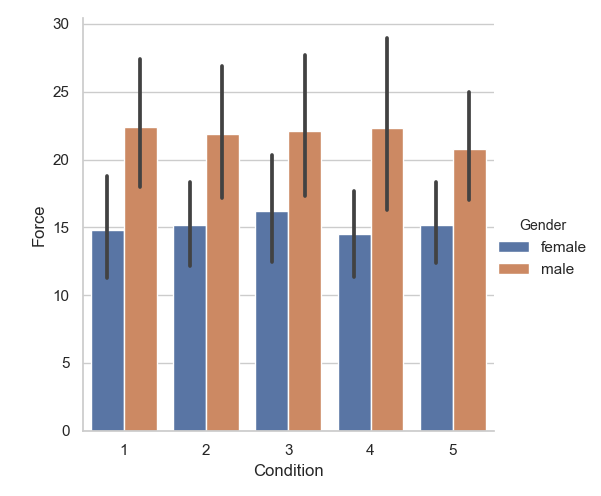
\includegraphics[scale=0.4]{Files/Plots/force_mean_by_condition__gen.png}
         \caption{Mean force.}
     \label{fig:forceMeanCondGen}
     \end{subfigure}
     \hspace{7mm}
     \begin{subfigure}[b]{0.3\textwidth}
         \centering
     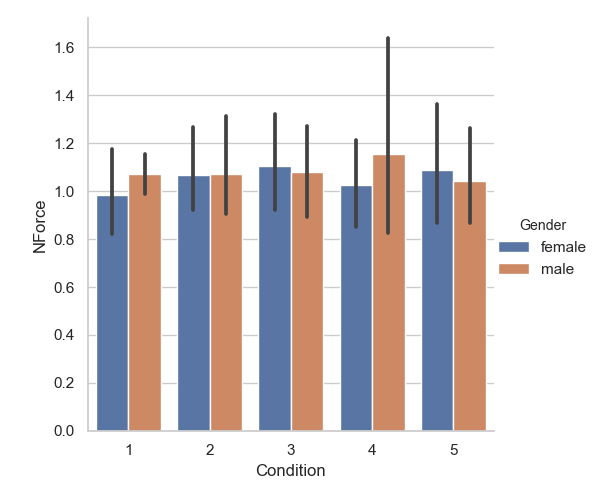
\includegraphics[scale=0.4]{Files/Plots/forceNforce_mean_by_condition_gen.png}
         \caption{Mean N1 force.}
     \label{fig:forceN1MeanGen}
     \end{subfigure}
        \hspace{7mm}
      \begin{subfigure}[b]{0.3\textwidth}
         \centering
     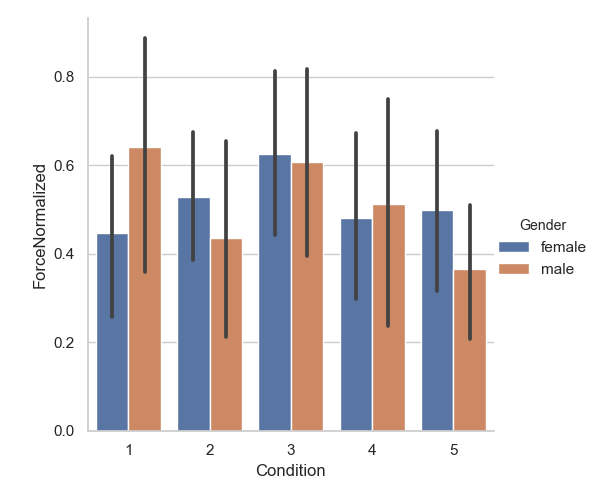
\includegraphics[scale=0.4]{Files/Plots/forceNormalized_mean_by_condition_gen.png}
         \caption{Mean N2 force.}
     \label{fig:forceN2MeanGen}
     \end{subfigure}
     \caption{Mean force, N1 , N2  by condition and by gender. Lines on bars denote confidence intervals.}
     \label{fig:forceMeanGenAll}
\end{figure} 
\begin{figure}[H]
\hspace{-10mm}
     \begin{subfigure}[b]{0.3\textwidth}
         \centering         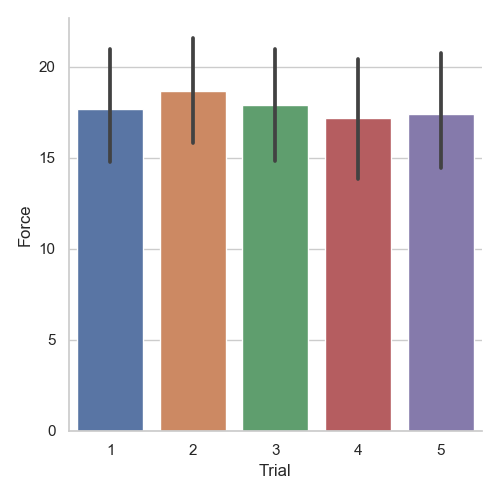
\includegraphics[scale=0.4]{Files/Plots/force_mean_by_trial.png}
         \caption{Mean force.}
     \label{fig:forceMeanTrial}
     \end{subfigure}
     \hspace{7mm}
     \begin{subfigure}[b]{0.3\textwidth}
         \centering
     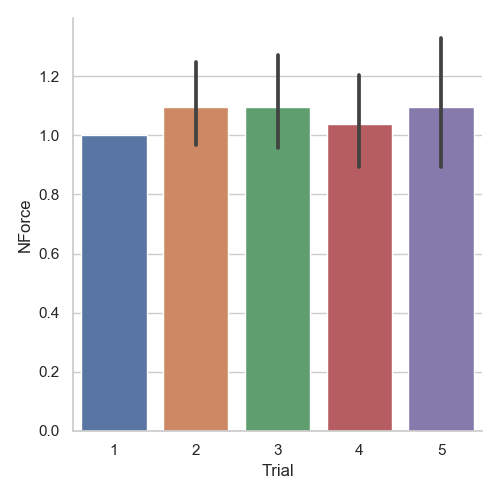
\includegraphics[scale=0.4]{Files/Plots/forceNforce_mean_by_trial.png}
         \caption{Mean N1 force.}
     \label{fig:forceN1Trial}
     \end{subfigure}
     \hspace{7mm}
      \begin{subfigure}[b]{0.3\textwidth}
         \centering
     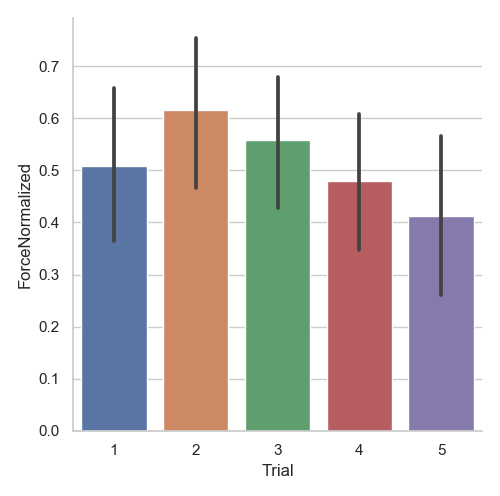
\includegraphics[scale=0.4]{Files/Plots/forceNormalized_mean_by_trial.png}
         \caption{Mean N2 force.}
     \label{fig:forceN2Trial}
     \end{subfigure} \\
     
     \hspace{-10mm}
     \begin{subfigure}[b]{0.3\textwidth}
\centering
     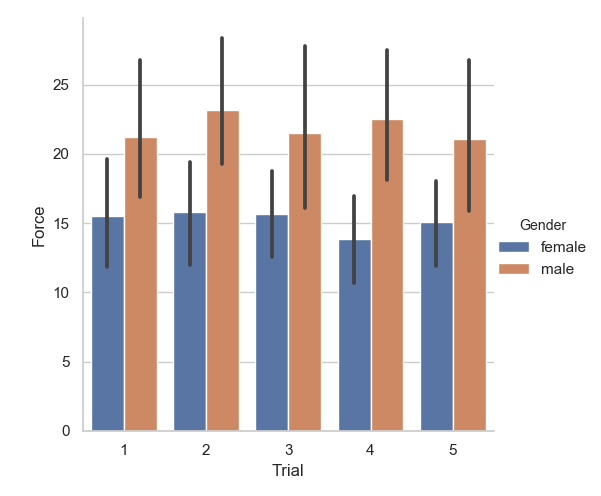
\includegraphics[scale=0.4]{Files/Plots/force_mean_by_trial_gen.png}
         \caption{Mean force.}
     \label{fig:forceMeanTrialGen}
     \end{subfigure}
    \hspace{7mm}
     \begin{subfigure}[b]{0.3\textwidth}
         \centering
     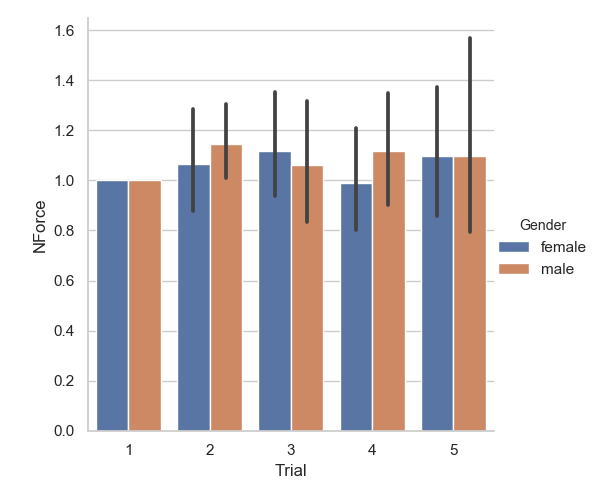
\includegraphics[scale=0.4]{Files/Plots/forceNforce_mean_by_trial_gen.png}
         \caption{Mean N1 force.}
     \label{fig:forceN1TrialGen}
     \end{subfigure}
     \hspace{7mm}
      \begin{subfigure}[b]{0.3\textwidth}
         \centering
     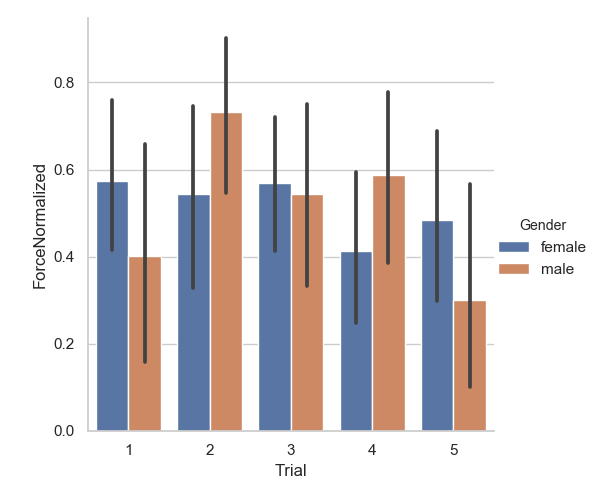
\includegraphics[scale=0.4]{Files/Plots/forceNormalized_mean_by_trial_gen.png}
         \caption{Mean N2 force.}
     \label{fig:forceN2TrialGen}
     \end{subfigure}
     \caption{Mean force, N1, N2  by trial, and by gender in the second row. Error bars show 95\%  confidence interval.}
     \label{fig:allForceTrial}
\end{figure} 
From figures displayed in \ref{fig:forceMeanGenAll} we can see males pulled more than females. Additionally, the error bars seem to be overall bigger for males than females. Error bars are biggest for N2 due to the normalization procedure, as minimum values are considered 0 and maximum values 1. Male participants seem to have the biggest error bars in condition 4.
\\
In figure \ref{fig:allForceTrial} we display our results by trial. Both males and females seemed to have pulled harder in the second trial. We look at the distributions of avatars per trial in order to determine if the effect is due to order or representation. Figure \ref{fig:condPerTrial} shows that in the third trial there were the most avatars in condition 3. The high pulling values would, therefore, more likely occur because of condition than trial order, as participants seemed to pull hardest for the average condition.
\\
 While an effect of ordering seems to be less strong than appearance, we observed some design issues for the first trial. Participants reacted in various ways due to the novelty of the experience or the setup. As such, we isolate the first trial to look for discernible differences.
 \\
 We examine our results considering only the first trial in figures  \ref{fig:meanF1st} and \ref{fig:meanF1stGen}. In figures \ref{fig:meanFRest} and \ref{fig:meanFRestGen} we look at our results excepting the first trial.  We notice there are 2 trends between these force pulls. In the first trial, womens' pull on the rope increases until the third condition, then decreases. They pull the least in condition 2, which was the avatar rated most strong and intimidating by women participants (see \ref{fig:weightedFEx}). There is only one data point for males in the average condition, which seems to be an outlier of very high force. It would explain the high value for condition 3 for all participants in figure \ref{fig:meanF1st}. Males' pull increases again for the last condition. When we consider trials 2,3,4 and 5 there is also an increase in pull for women in condition 5. Overall it looks like the first trial has an uptick in the force for the average condition, something not present when considering only the last 3 trials.\\


\begin{figure}[H]
 \begin{subfigure}[b]{0.5\textwidth}
     \centering
     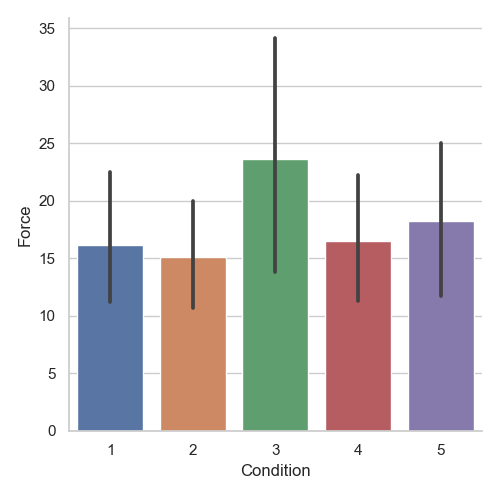
\includegraphics[scale=0.5]{Files/Plots/force_in_first_trial.png}
     \caption{Mean force in 1st trial.}
     \label{fig:meanF1st}
 \end{subfigure}
  \begin{subfigure}[b]{0.5\textwidth}
     \centering
     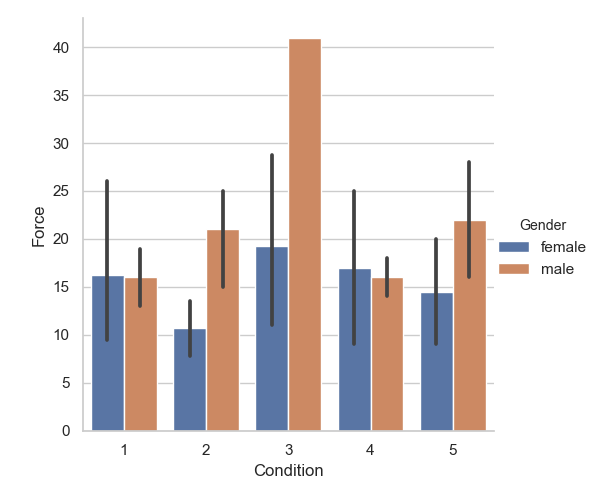
\includegraphics[scale=0.5]{Files/Plots/force_first_gen.png}
     \caption{Mean force in first trial gendered.}
     \label{fig:meanF1stGen}
 \end{subfigure}
  \begin{subfigure}[b]{0.5\textwidth}
     \centering
     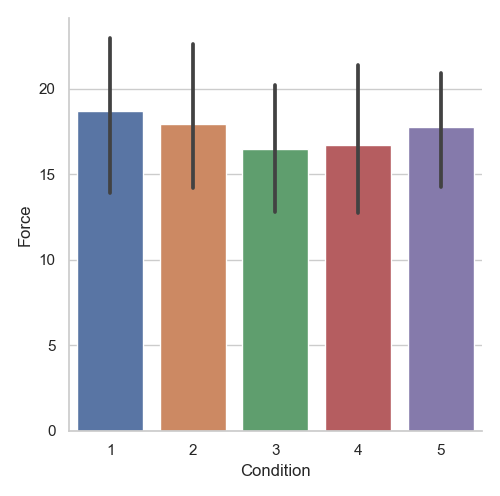
\includegraphics[scale=0.5]{Files/Plots/force_all_but_1.png}
     \caption{Mean force in all trials except first one.}
     \label{fig:meanFRest}
 \end{subfigure}
     \begin{subfigure}[b]{0.5\textwidth}
     \centering
     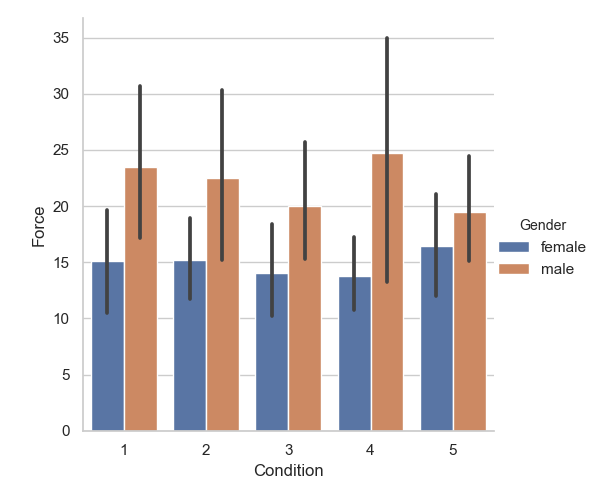
\includegraphics[scale=0.5]{Files/Plots/forc_all_but_1_gen.png}
     \vspace{-5mm}
     \caption{Mean force in all trials except the first one  gendered.}
     \vspace{-5mm}
     \label{fig:meanFRestGen}
 \end{subfigure}
 \vspace{1mm}
     \caption{Mean force by condition and by gender, taken for the first and first 3 trials. Error bars show 95\%  confidence interval.}
    \label{fig:forceIn1stRest}
\end{figure}
\begin{figure}[H]
\hspace{-10mm}
 \captionsetup{justification=centering,margin=0.1cm}
 \centering
 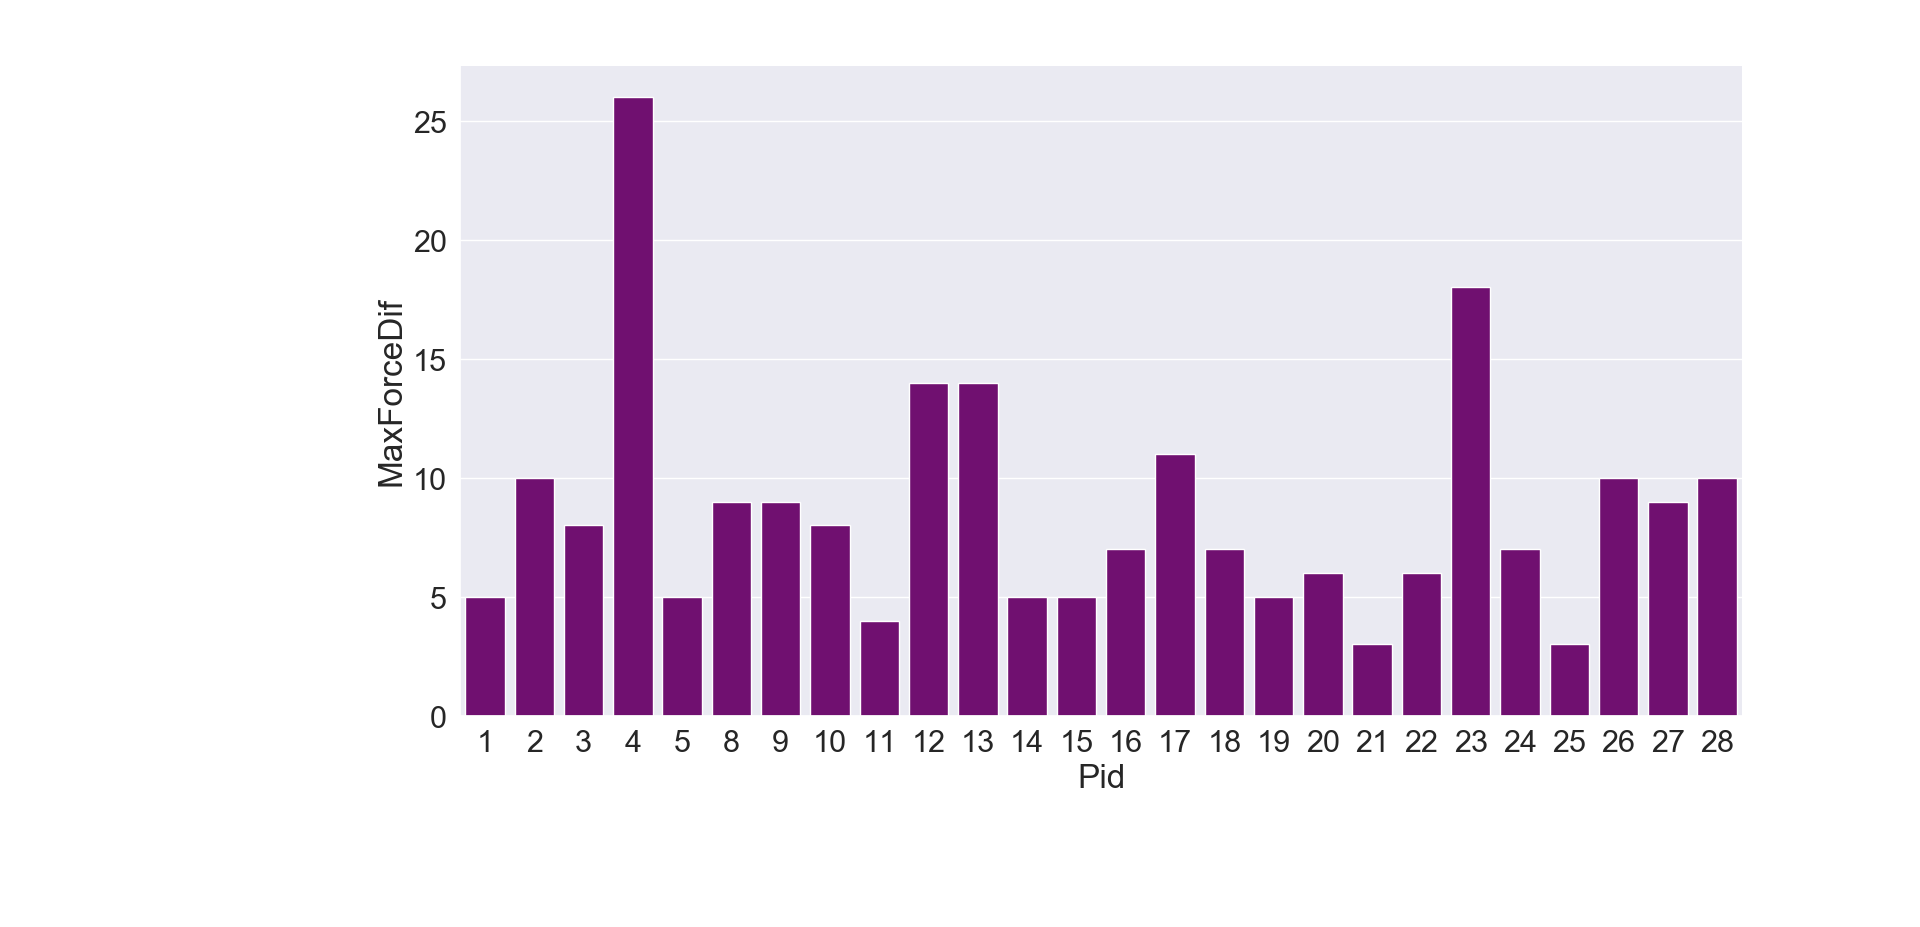
\includegraphics[width=\linewidth]{Files/Plots/max_force_dif.png}
 \caption{Maximum force difference per participant.}
\label{fig:forceDif}
\end{figure} 
Participants did not appear to use force in accordance with our hypotheses (H2). However, our data shows some users varied their pull very much.
We explore the maximum differences in pulling for each participant in figure \ref{fig:forceDif}. On average, the difference was: $M=8.61538, SD=4.94995$. However, there are several outliers. The maximum pull difference was for participant 4 --- 26 kg of force. With our hypothesis, we presumed there would be differences in pulling, however such large differences suggest participants were not simply reacting to their opponent. Rather, some other factors seem to have influenced their pull strategies. Qualitative feedback offers some insight into this behavior. These large variations support our observations that participants tested the application. They behaved in an unexpected way in order to test their own assumptions about the opponents, not always respecting the instructions of the experimenter.\\
\\
\textbf{Discussion}\\
 From qualitative feedback we also noticed that, as participants carry on with the rope-pulling, the illusion that the rope is being pulled eventually breaks. This suggests there might be a trend of lower force across trials. Figure \ref{fig:allForceTrial} shows some indication of a downwards trend for mean force and N2. Another explanation could be that participants simply felt tired and pulled less. A correlation between performance and realism should be explored in future research. Keeping the number of trials at a minimum to avoid fatigue should be considered a priority. 
\\
Nass et al. put forward the social response theory  known as \textit{Computers Are Social Actors} (CASA). Their observations have shown that people treat computers as social actors \cite{nass1994computers}. Essentially, it means that people conform to social rules throughout their interactions and behave towards a computer as they would towards another human. Furthermore, people seem to mindlessly apply these social rules and other expectations in this context. Some examples are: attributing social categories as gender stereotypes, increased reciprocity in response to assistance,  self disclosure reciprocity. We can explain our participants' expectations in terms of the CASA paradigm. People expect strong people to pull harder in real life, so this expectation was projected onto virtual humans and its associated force \textit{mechanism}. It seems clear from our feedback that people assumed there was a machine, and only one, which provided the force and the virtual humans were meant to be representations of this force. 
\\
Another reason why we expected participants to pull harder was due to the priming effect of avatars' appearances, similar with \cite{pena2009priming}. Aggressive cues were meant to activate peoples' aggressive behavior and enable them to pull stronger. Considering the interplay between these psychological effects, we expected a similar outcome for our experiment, that people would pull stronger for strong avatars. Our results, however, our results are inconclusive. They capture the variability of human behavior.
\\
Social comparison theory posits people judge their qualities with respect to the perceived attributes of others. Peña and colleagues  frame their results for exergames performance in terms of this theory and note that weight did not solely have a significant effect, but rather the observed differences were a result of an interplay between avatars' and agents appearance' \cite{pena2016see}. Some qualitative feedback suggests participants were comparing themselves to the opponents, especially relative to size. Thus, assuming they would pull less with less stronger looking avatars would be in conformity with this theory.  We considered that participants could be intimidated by the strong avatars and thus pull less due to inhibition. From qualitative feedback, avatars did not seem to generate enough realism for participants to react in this manner. Participants remarked being spurred into action by strong appearances, as opposed to being put off.
\\
 From a Protean perspective, participants' avatars were bigger than the weaker opponents. This could explain why users tended to pull stronger in the weakest conditions. By the self-perception paradigm, users would see themselves stronger and as such perform stronger. An issue with adopting a Protean perspective for this research is that participants did not see themselves in a virtual mirror before the game, as with usual Proteus Effect studies \cite{bailenson2006transformed}. Furthermore, they did not appear to look at their arms nearly as much as they looked at their opponents, as shown in figure \ref{fig:gazePie}. However, we postulate that the novelty of the experience and ambiguity determined participants to act in a way that is not natural. After all, playing tug-of-war with a virtual person in a virtual environment is not a natural, commonplace experience. Furthermore, participants also mentioned restraining themselves in various ways, by keeping their legs still or being careful not to pull too hard. These actions might determine high cognitive load preventing a natural social response. Despite this, the general consensus among researchers seems to be that VR can generate realistic reactions and is ideal to study psychological and social behavior without endangering participants \cite{fox2009virtual}.
 \\
The large force variations make our measurements unreliable to support hypothesis H2. This is especially true for some participants with a very big difference in pull. If users have different motivations for pulling stronger than simply reacting to their opponent, we cannot make a reliable case for our research aims. Moreover, testing the application suggests that participants did not follow the instructions provided by the experimenter. We do not know what effect this could have on their perceived pull value, but we speculate participants could have overcompensated in cases in which they pulled much less. We believe there is a reasonable doubt to be shed over the measures for H2 and H3. We cannot and should not prevent participants from using our systems in playful and unexpected ways. This behavior is documented for other new technologies such as conversational agents \cite{jain2018evaluating}. For a question-answering system, Liao et al. document similar playful and curiosity-driven behavior. Approximately 85\% of users asked the system questions outside the scope of its advertised purpose \cite{liao2018all}. For games or VR experiences meant to give rise to VR illusions, we suggest extensive piloting in order to establish users' expectations. This would allow for more realistic interactions with the system and reduce the number of breaks in presence or plausibility.  

 \clearpage   
\subsubsection{Perceived Pull and Challenge}
\label{subsubsection:ppullChallenge}
%%%%%%%%%%%%%%%%%%%%%%%%%%%%%%%%%%%%%%%%
%               CHALLENGE ppull counts
%%%%%%%%%%%%%%%%%%%%%%%%%%%%%%%%%%%%%%%
  
\begin{figure}[H]
\centering
\captionsetup{justification=centering,margin=0.1cm}
\hspace{-20mm}
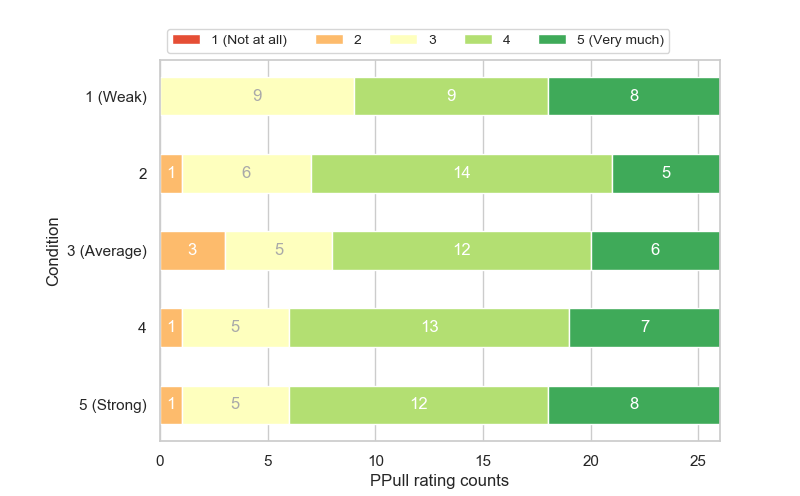
\includegraphics[scale=0.7]{Files/Plots/ppull_by_condition_count_stacked.png}
\caption{Count of perceived pull ratings by condition.}
\label{fig:ppullStacked}
\end{figure}
\vspace{-5mm}

\begin{figure}[H]
\captionsetup{justification=centering,margin=0.1cm}
 \centering
 \hspace{-20mm}
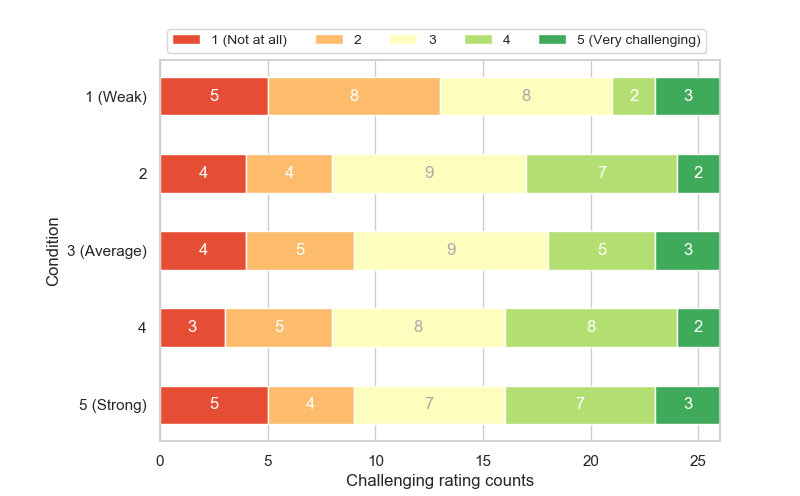
\includegraphics[scale=0.7]{Files/Plots/challenge_by_condition_count_staked.png}
\caption{Count of challenge ratings by condition.}
\label{fig:challengeStacked}
\end{figure}
\pagebreak
The majority of participants seemed to rate opponents with different challenges, which gives support to H1. Their reported values do not seem to coincide with our assumptions from H2 and H3.
\\
\textbf{Results}\\
Above in figures \ref{fig:ppullStacked} and 
\ref{fig:challengeStacked} we present an overview for the ratings given to Q3 and Q4 between rope-pulls, namely challenge and perceived pull (see \ref{enum:panelQuestions}). 
\begin{itemize}
\itemsep0em
 \item \textbf{Q3}: How much did you pull the rope? Rating: 1 (\textit{Not at all}), to 5 (\textit{Very much});
\item \textbf{Q3}: How challenging was this round? Rating: 1 (\textit{Not at all}), to 5 (\textit{Very challenging}).
\end{itemize}
To see the total ratings for these metrics per participants, please refer to section \ref{subsection:heatmap}, for perceived pull (\ref{fig:ppullHeatmap}) and challenge (\ref{fig:challengeHeatmap}).

%%%%%%%%%%%%%%%%%%%%%%%%%%%%%%%%%%%%%%%%
%               CHALLENGE
%%%%%%%%%%%%%%%%%%%%%%%%%%%%%%%%%%%%%%%
\begin{figure}[H]
 \begin{subfigure}[b]{0.5\textwidth}
     \centering
     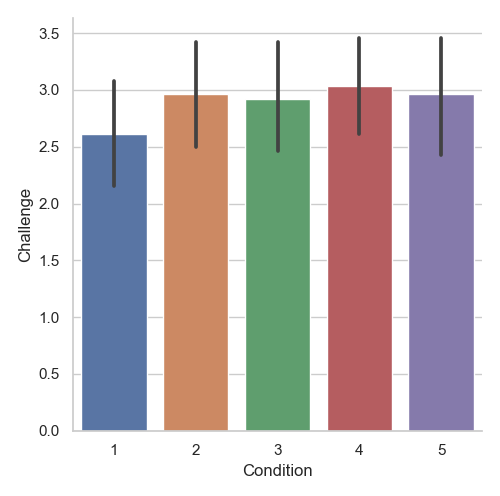
\includegraphics[scale=0.5]{Files/Plots/challenge_by_condition_mean.png}
     \caption{Mean challenge by condition.}
     \label{fig:meanChal}
 \end{subfigure}
  \begin{subfigure}[b]{0.5\textwidth}
     \centering
     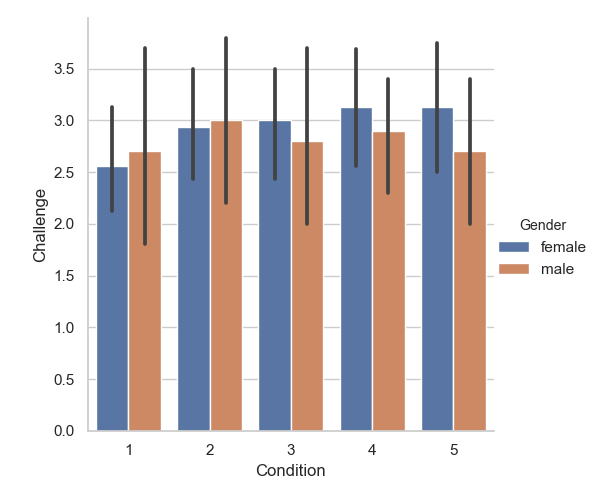
\includegraphics[scale=0.5]{Files/Plots/challenge_by_condition_mean_gen.png}
     \caption{Mean challenge by condition gendered.}
     \label{fig:meanChalGen}
 \end{subfigure}
     \caption{Mean challenge by condition, and by gender. Error bars show 95\%  confidence interval.}
    \label{fig:chalByCond}
\end{figure}
Most participants did give different ratings across trials, despite the rope having the same resistance ($M=2.9,\; SD=1.21265 $), which appears to support \textbf{H1}. In tables \ref{tabular:meanChalCond} and \ref{tabular:meanChalTrial} we display the means and standard deviation of challenge ratings by condition and trial respectively.
Figure \ref{fig:chalByCond} shows mean challenge given by participants for each condition. In womens' case, it would appear to support our hypothesis, however women rated condition 2 as being strongest. Males had a downward trend when rating challenge. However, the confidence intervals for some condition indicate large variation. We can see in table \ref{tabular:meanChalCond} that condition 5 had the highest standard deviation.

\begin{table}[H]
 \captionsetup{justification=centering,margin=0.1cm}
 \begin{minipage}{.5\linewidth}
     \centering
\begin{tabular}{|lll|}
\hline
Cond & Mean & SD \\
\hline
1 & 2.61538 & 1.23537\\  
2 &  2.96153 & 1.18256\\ 
3 &  2.92307 & 1.23038\\ 
4 &  3.03846 & 1.14824\\  
5 & 2.96153 & 1.31090\\  
\hline
\end{tabular}
\caption{Mean challenge and standard deviation by condition.}
\label{tabular:meanChalCond}
\end{minipage}\hfill
 \begin{minipage}{.5\linewidth}
 \centering
\begin{tabular}{|lll|}
\hline
Trial & Mean & SD \\
\hline
1 & 2.5 & 1.1401\\  
2 & 2.92307 & 1.23038\\  
3 & 3.15384 &  1.28661\\  
4 & 2.96153 & 1.11286\\  
5 & 2.96153 & 1.28002\\  
\hline
\end{tabular}
\caption{Mean challenge and standard deviation by trial.}
\label{tabular:meanChalTrial}
\end{minipage}
\label{tbl:meanChalCond1}
\end{table} 

\begin{figure}[H]
 \begin{subfigure}[b]{0.5\textwidth}
     \centering
     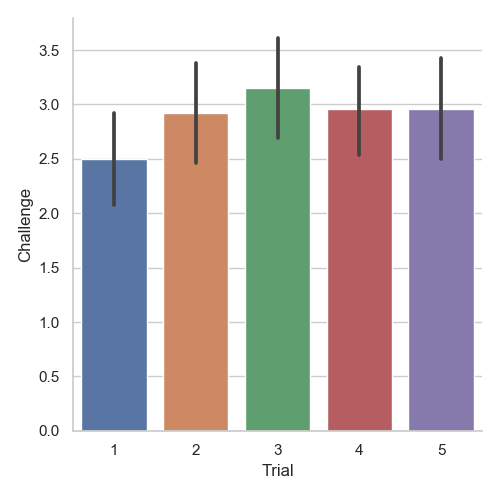
\includegraphics[scale=0.5]{Files/Plots/challenge_by_trial_mean.png}
     \caption{Mean challenge by trial.}
     \label{fig:meanChalTrial}
 \end{subfigure}
  \begin{subfigure}[b]{0.5\textwidth}
     \centering
     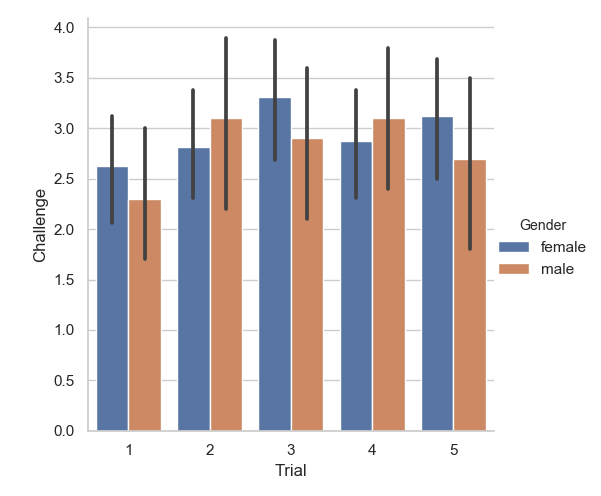
\includegraphics[scale=0.5]{Files/Plots/challenge_by_trial_median_gen.png}
     \caption{Mean challenge by trial gendered.}
     \label{fig:meanChalTrialGen}
 \end{subfigure}
     \caption{Mean challenge by trial, and by gender. Error bars show 95\%  confidence interval.}
    \label{fig:chalByTrial}
\end{figure}

Figure \ref{fig:chalByCond} shows
mean challenge ratings by trial. We can see the challenge increase until the second trial for males, and until the third trial for females. Results seem to vary more by trial which could support our observation that appearance had a stronger effect than ordering.
We inspect the results for the first trial only in figure \ref{fig:Chal1st} below. These results seem to vary with the first condition being rated more challenging overall by males and females. The challenge ratings for the first trial seem to follow a similar trend as the force values. We note that in the first trial there were more avatars in condition 1 and 2 which could suggest an effect of over-representation. 
\\ We observed that participants did not use the same standard for the challenging rating. Furthermore, some changed their assumptions dynamically during the game, based on visual feedback or their internal state. We detail these observations in section \ref{qualitativeFeedback}. A limitation is that we did not gather the assumptions participants had about this rating, however we noted their voluntary comments.

\begin{figure}[H]
 \begin{subfigure}[b]{0.5\textwidth}
     \centering
     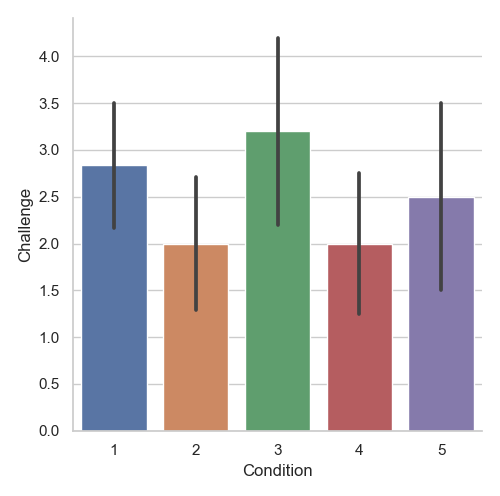
\includegraphics[scale=0.5]{Files/Plots/challenge_first_trial.png}
     \caption{Mean challenge for 1st trial.}
     \label{fig:meanChal1st}
 \end{subfigure}
  \begin{subfigure}[b]{0.5\textwidth}
     \centering
     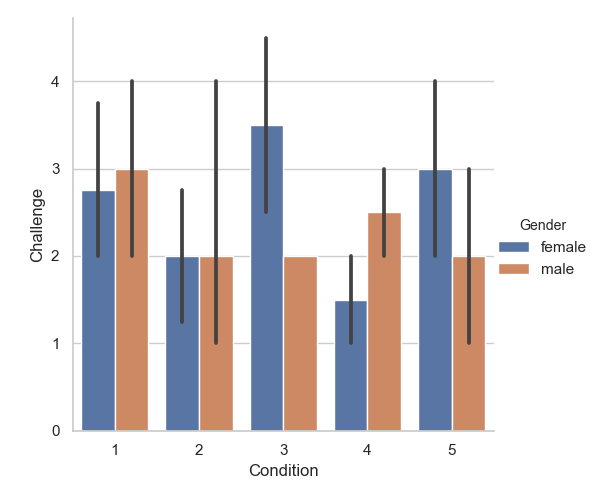
\includegraphics[scale=0.5]{Files/Plots/challenge_first_trial_gen.png}
     \caption{Mean challenge for 1st trial gendered.}
     \label{fig:meanChalGen1st}
 \end{subfigure}
     \caption{Mean challenge by condition, and by gender for first trial. Error bars show 95\%  confidence interval.}
    \label{fig:Chal1st}
\end{figure}

%%%%%%%%%%%%%%%%%%%%%%%%%%%%%%%%%%%%%%%%
%               ppull
%%%%%%%%%%%%%%%%%%%%%%%%%%%%%%%%%%%%%%%

The majority of participants also reported pulling differently, despite competing in a game to pull the strongest ($ M=3.93846,\; SD=0.82362 $). In tables \ref{tbl:meanPPullCond} and \ref{tbl:meanPPullTrial} we show the mean perceived pulls by condition and trial. Participants seemed to pull stronger in the last conditions, despite rating them less challenging. It appears they were also more consistent with their answers in this metric, as standard deviation for is less for perceived pulls.

\begin{table}[H]
 \captionsetup{justification=centering,margin=0.1cm}
 \begin{minipage}{.5\linewidth}
     \centering
\begin{tabular}{|lll|}
\hline
Cond & Mean & SD \\
\hline
1 &  3.96153 & 0.82368\\  
2 &  3.88461 & 0.76560\\ 
3 &  3.80769 & 0.9389\\ 
4 &  4.0 & 0.8\\  
5 & 4.03846 & 0.8236\\  
\hline
\end{tabular}
\caption{Mean perceived pull and standard deviation by condition.}
\label{tbl:meanPPullCond}
\end{minipage}\hfill
 \begin{minipage}{.5\linewidth}
 \centering
\begin{tabular}{|lll|}
\hline
Trial & Mean & SD \\
\hline
1 & 3.73076 & 0.82741\\  
2 & 4.15384 & 0.6748\\  
3 & 3.76923 &  0.99227\\  
4 & 3.92307 & 0.7961\\  
5 & 4.11538 &  0.76560\\  
\hline
\end{tabular}
\caption{Mean perceived pull and standard deviation by trial.}
\label{tbl:meanPPullTrial}
\end{minipage}
\end{table} 

In figure \ref{fig:ppullByCond}, below, we show mean perceived pull values by condition and trial. By condition there seems to be a trend for the perceived pull. Namely that it seems to decrease until the average condition then increase again. This trend could support our hypothesis, namely that participants believed they pulled more for stronger-looking avatars. 
\\
The challenges and perceived pulls show two different trends. While challenges seem to peak at the average condition and look similar to the actual force, perceived pulls appear to decrease at condition 3.

\begin{figure}[H]
 \begin{subfigure}[b]{0.5\textwidth}
     \centering
     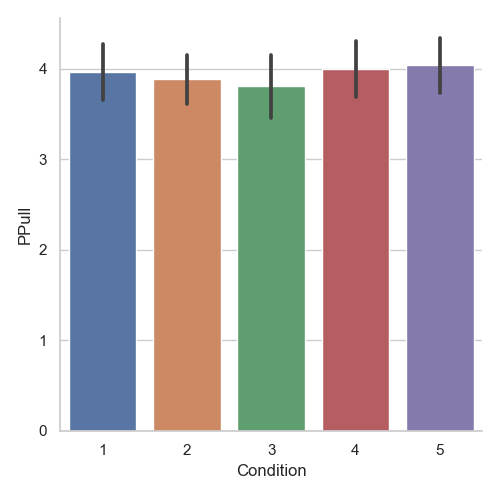
\includegraphics[scale=0.5]{Files/Plots/ppull_by_condition_mean.png}
     \caption{Mean perceived pull by condition.}
     \label{fig:meanPPullCond}
 \end{subfigure}
  \begin{subfigure}[b]{0.5\textwidth}
     \centering
     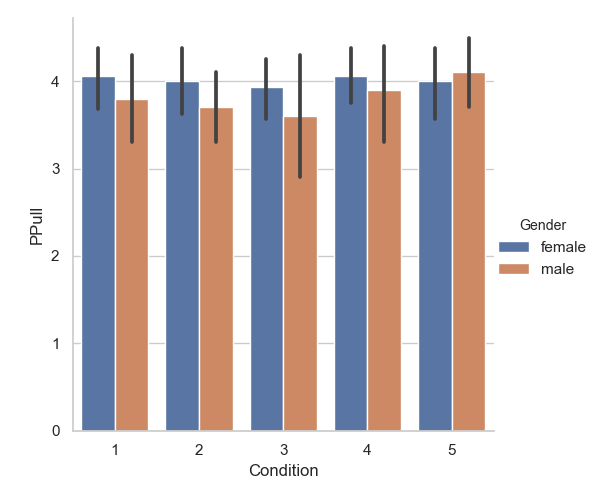
\includegraphics[scale=0.5]{Files/Plots/ppull_by_condition_median_gen.png}
     \caption{Mean ppull by condition gendered.}
     \label{fig:fig:meanPPullGenCond}
 \end{subfigure}
     \caption{Mean perceived pull by condition, and by gender. Lines on bars denote confidence intervals.}
    \label{fig:ppullByCond}
\end{figure}
In figure \ref{fig:ppullByTrial} we show the mean perceived pull by trials. Seems participants thought they pulled strongest in the second and last trials. Overall, they reported less perceived strength for the first trial.

 \begin{figure}[H]
 \begin{subfigure}[b]{0.5\textwidth}
     \centering
     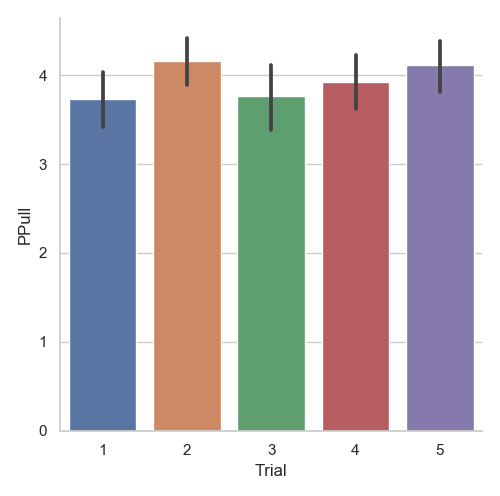
\includegraphics[scale=0.5]{Files/Plots/ppull_by_trial_mean.png}
     \caption{Mean perceived pull by trial.}
     \label{fig:meanPpullTrial}
 \end{subfigure}
  \begin{subfigure}[b]{0.5\textwidth}
     \centering
     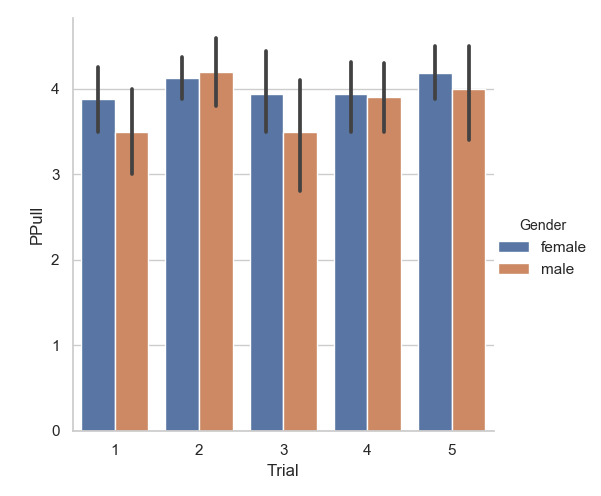
\includegraphics[scale=0.5]{Files/Plots/ppull_by_trial_mean_gen.png}
     \caption{Mean perceived pull by trial gendered.}
     \label{fig:meanPPullGenTrial}
 \end{subfigure}
     \caption{Mean perceived pull by trial, and by gender.  Error bars show 95\%  confidence interval.}
    \label{fig:ppullByTrial}
\end{figure}


\begin{figure}[H]
 \begin{subfigure}[b]{0.5\textwidth}
     \centering
     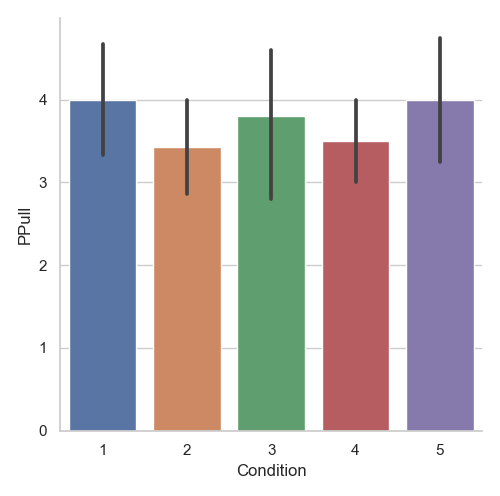
\includegraphics[scale=0.5]{Files/Plots/ppull_first_trial.png}
     \caption{Mean perceived pull for 1st trial.}
     \label{fig:meanPPull1st}
 \end{subfigure}
  \begin{subfigure}[b]{0.5\textwidth}
     \centering
     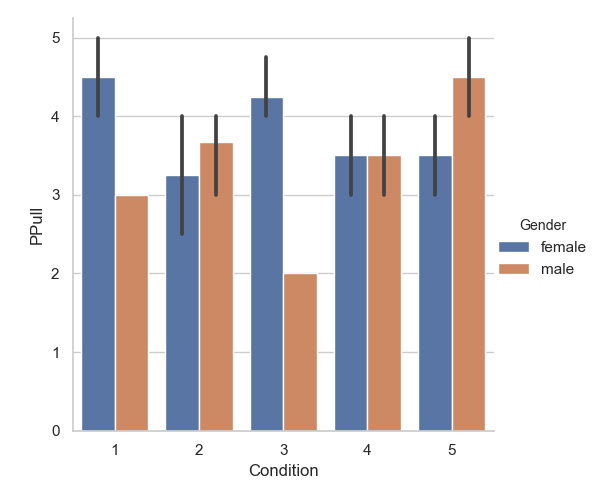
\includegraphics[scale=0.5]{Files/Plots/ppull_first_trial_gen.png}
     \caption{Mean ppull for 1st trial gendered.}
     \label{fig:meanPPullGen1st}
 \end{subfigure}
     \caption{Mean perceived pull by condition, and by gender for first trial. Error bars show 95\%  confidence interval.}
    \label{fig:PPull1st}
\end{figure}
We also look at the perceived pulls only for the first trial in figure \ref{fig:PPull1st}. Again, they seem to differ from the overall trend, but appear similar to the reported challenges for the first trial. However, there is only one data point for males in condition 1 and 3.
\\
\\
\textbf{Discussion}\\
It seems that the results do not show support for hypotheses H3 and H4. The trends they show, however, lead us to believe that H3 and H4 should not be dismissed. Perceived pulls seem to conform the most with our hypothesis so far.
\\
\\
Our observations that the illusion seemed to break as the game went on would lead us to believe participants behaved more realistically in the first few trials. This lead us to look at the isolated results. 
Force, perceived pull and challenge measurements do not seem to show a consistent trend. What is interesting, however, is that isolating results only for the first trial seems to paint the same picture of the data. Condition 3 seems to be the highest rated and measures, and the extremities (condition 1 and 5) show a slight increase.
\\
As values for perceived pull and challenge seem to increase for the last conditions, it seems less likely participants would be intimidated by the opponents into pulling less. We also suggest, based on our feedback, that the behavior of the agents was not realistic enough to determine such a response. Participants noticed their opponents did not react in sync with their pulling. Increasing realism could determine participants to respond more naturally.  However, increasing behavior realism of the  virtual humans can give rise to uncanniness if not realized in a proper way \cite{brenton2005uncanny,stein2019stay}. 
\\
While \cite{fox2015avatars,pena2016see} found that opponent and avatar appearance mitigates task performance, we do not find any conclusive evidence to support our hypothesis. Since some participants changed their force pulling strategies, this inevitably must have affected their perceived pull.

Slater discusses the sustaining these illusions. He mentions that sustaining the illusion might depend on its credibility and conformity to expectations. \cite{slater2009place}

\subsubsection{Rope Agency and Realism}
\label{subsubsection:ropeOwnRealism}
%%%%%%%%%%%%%%%%%%%%%%%%%%%%%%%%%%%%%%%%
%               rope ownership
%%%%%%%%%%%%%%%%%%%%%%%%%%%%%%%%%%%%%%%

Below we briefly present the results of the ratings for rope realism and agency (see Q1, Q2 in \ref{enum:panelQuestions}). While we are partially interested in these results, they serve to confirm our qualitative feedback that participants were generally a \textit{fan} of the rope. They rated rope agency highly 
($M=4.63846, \; SD=0.59720$), despite noticing inaccuracies in their hands representation. The same applies to rope realism ($M=4.51538, \; SD=0.58713$), in figure \ref{fig:ropeOwnershipRealism}. In general, participants found the rope to behave as a real rope.

\begin{figure}[H]
 \begin{subfigure}[b]{0.3\textwidth}
     \centering
     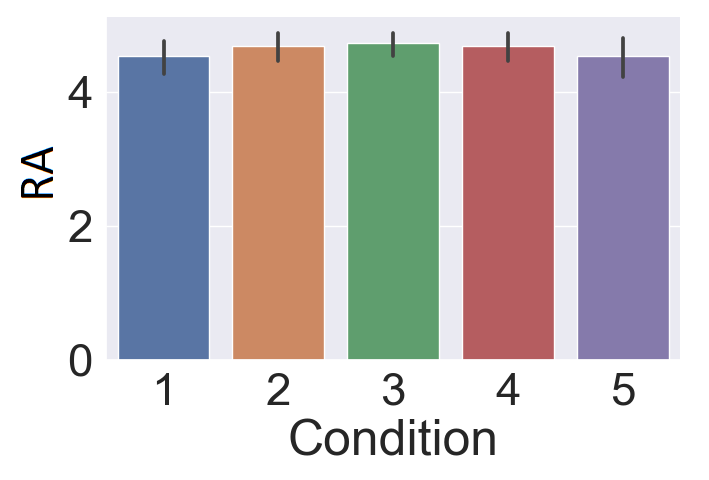
\includegraphics[scale=0.3]{Files/Plots/rocond.png}
     \caption{Mean rope agency by condition.}
     \label{fig:ropeOwnCond}
 \end{subfigure}
  \begin{subfigure}[b]{0.3\textwidth}
     \centering
     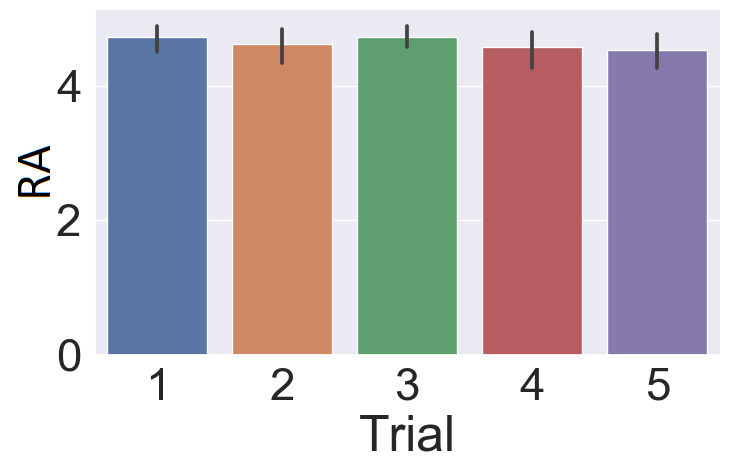
\includegraphics[scale=0.3]{Files/Plots/rotrial.png}
     \caption{Mean rope agency by trial.}
     \label{fig:ropeOwnTrial}
 \end{subfigure}
 \begin{subfigure}[b]{0.3\textwidth}
     \centering
     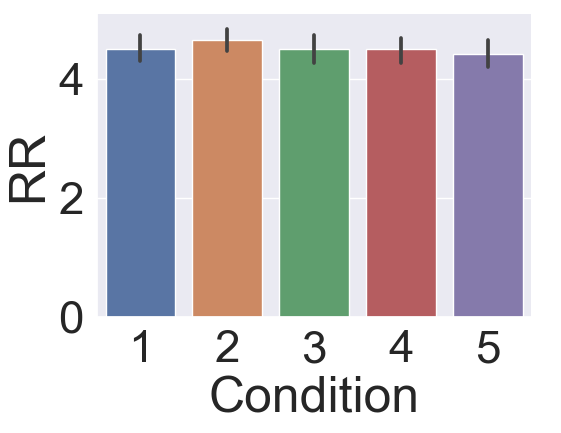
\includegraphics[scale=0.35]{Files/Plots/rrcond.png}
     \caption{Mean rope realism by condition.}
     \label{fig:ropeRealCond}
 \end{subfigure}
 \hspace{-5mm}
  \begin{subfigure}[b]{0.3\textwidth}
     \centering
     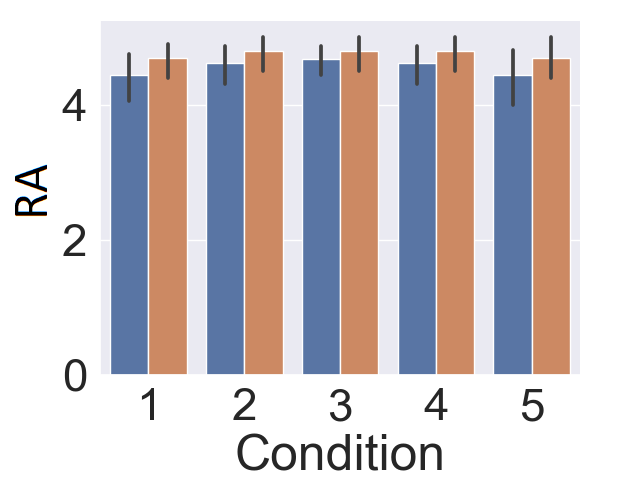
\includegraphics[scale=0.3]{Files/Plots/rocond_gen.png}
     \caption{Mean rope agency by condition gendered.}
     \label{fig:ropeOwnCondGend}
 \end{subfigure}
   \begin{subfigure}[b]{0.3\textwidth}
     \centering
     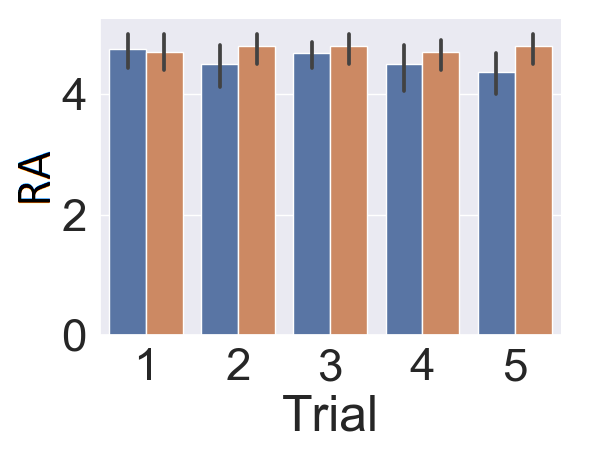
\includegraphics[scale=0.3]{Files/Plots/rotrial_gen.png}
      \caption{Mean rope agency by trial gendered.}
     \label{fig:ropeOwnTrialGend}
 \end{subfigure}
  \hspace{5mm}
  \begin{subfigure}[b]{0.3\textwidth}
     \centering
     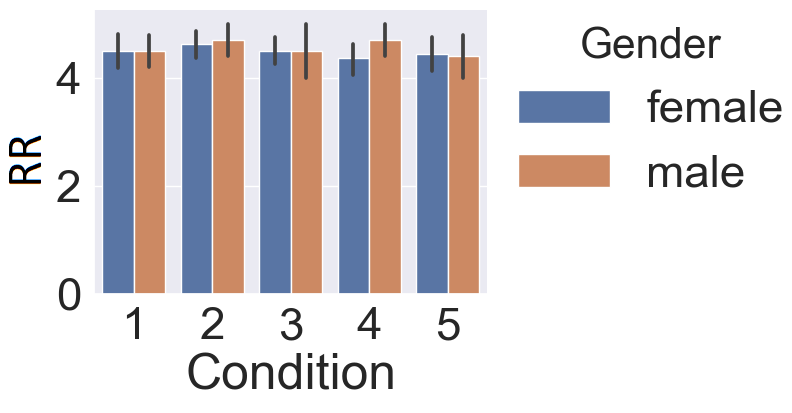
\includegraphics[scale=0.35]{Files/Plots/rrcond_gen.png}
     \caption{Mean rope realism by condition gendered.}
     \label{fig:ropeRealCondGend}
 \end{subfigure}
     \caption{Mean rope agency and rope realism by condition, trial, and by gender. Error bars show 95\%  confidence interval.}
    \label{fig:ropeOwnershipRealism}
\end{figure}

\textbf{Discussion}
\\
For males it suggests by the challenges they were intimidated.

%%%%%%%%%%%%%%%%%%%%%%%%%%%%%%%%%%%%%%%%
%               rope realism
%%%%%%%%%%%%%%%%%%%%%%%%%%%%%%%%%%%%%%%

\clearpage

\subsubsection{Post-experimental Survey Results}

In the following, error bars show standard deviation.
%%%%%%%%%%%%%%%%%%%%%%%%%%%%%%%%%%%%%%%%
%           misc all    %%%%%%%%%%%%%%%%%%%%%%%%%%%%%%%%%%%%%%%
\begin{figure}[H]
 \centering
 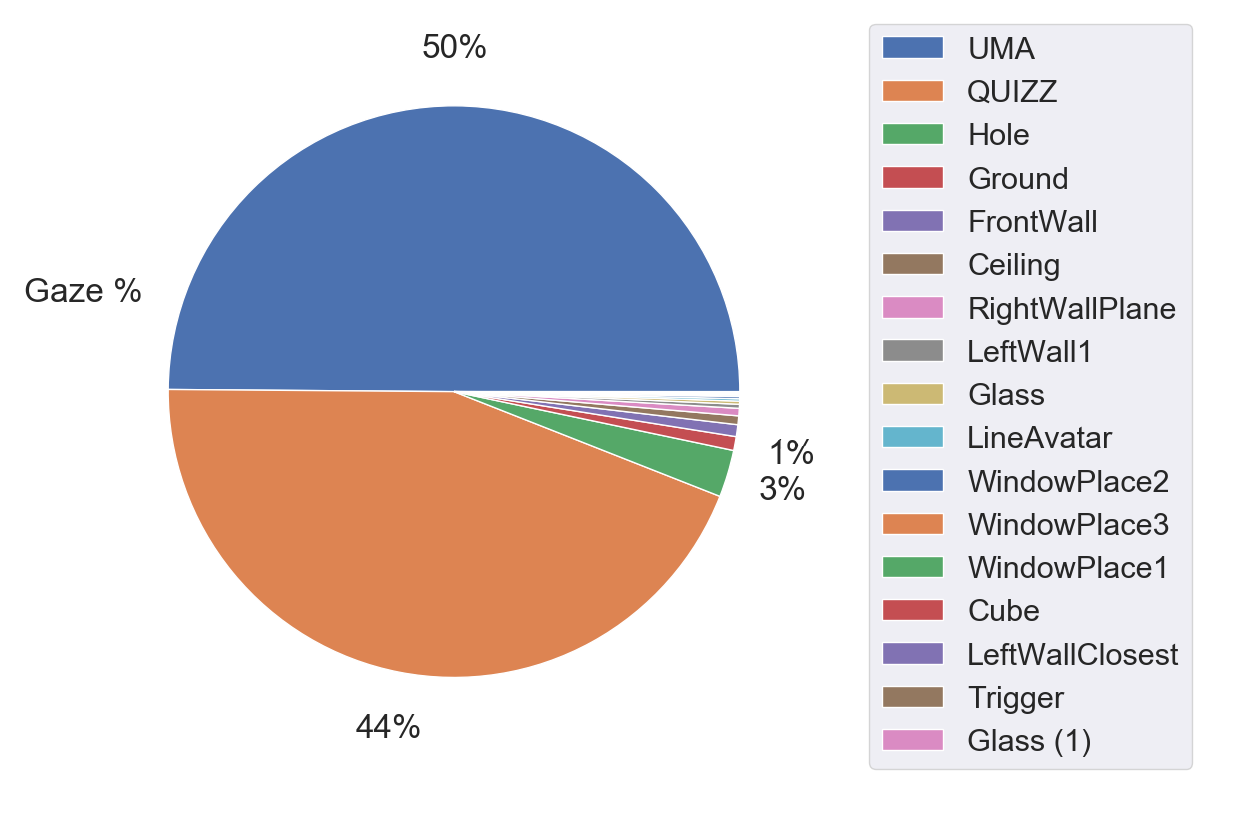
\includegraphics[scale=0.5]{Files/Plots/gaze_plots.png}
 \caption{Percent participants gazed at objects during the whole experiment duration. }
\label{fig:gazePie}
\end{figure}
We did not have eye tracking, however we used the midpoint of the headset to estimate what objects participants were looking at. From figure \ref{fig:gazePie} it can be seen that participants mostly gazed at their opponents. The second most gazed object is the quiz panel (\textit{QUIZZ}), which is expected as participants were answering the questions written on it.  The arms were not tagged with a separate ID due to implementation. However, the object behind the hands was logged which would most likely be the \textit{Hole} or the \textit{Ground}. This is a rough estimation, however it is supported by qualitative data, the ratings for rope realism and rope ownership, which were generally very high despite inaccuracies in arm tracking.\\ 
\\
In figures \ref{fig:miscAll} below, we present all mean ratings for the co-presence ($M=3.53842,\;$ $ SD=0.99604 $), presence ($M=3.51538,\; SD=0.97849 $) and arm ownership ($M=3.69871,\; SD=1.26804 $) ratings. In figures \ref{fig:miscAllFemales} and \ref{fig:miscAllMales} we show the ratings for females and males respectively. Despite feedback that avatars were not expressive enough from several participants, co-presence mean does not differ significantly from the other categories. Among them, participants varied the most rating arm ownership. In what follows we give an overview of the post-experimental survey data by question. Please see tables \ref{tbl:pres}, \ref{tbl:copres} and \ref{tbl:own} for mean, median and standard deviation values for presence, co-presence and arm ownership.
\begin{figure}[H]
 \centering
 \hspace{-25mm}
 \begin{subfigure}[b]{0.5\textwidth}
 \includegraphics[scale=0.45]{Files/Plots/misc_all_mean.png}
 \caption{Total mean ratings.}
\label{fig:miscAll}
\end{subfigure}
 \hspace{20mm}
\begin{subfigure}[b]{0.5\textwidth}
 \centering
 \includegraphics[scale=0.45]{Files/Plots/misc_all_mean_f.png}
 \caption{Females mean ratings. }
 \label{fig:miscAllFemales}
 \end{subfigure}
  \hspace{10mm}
\begin{subfigure}[b]{1\textwidth}
 \centering
 \includegraphics[scale=0.45]{Files/Plots/misc_all_mean_m.png}
 \caption{Males mean ratings.}
 \label{fig:miscAllMales}
 \end{subfigure}
 \caption{Total mean co-presence, presence and ownership ratings by gender. Error bars show standard deviation. }
\label{fig:miscAllGendered}
\end{figure}


%%%%%%%%%%%%%%%%%%%%%%%%%%%%%%%%%%%%%%%%
%             copresence
%%%%%%%%%%%%%%%%%%%%%%%%%%%%%%%%%%%%%%%

\begin{figure}[H]
\hspace{-15mm}
\begin{subfigure}[b]{0.5\textwidth}
 \centering
 \includegraphics[scale=0.5]{Files/Plots/copresence_mean.png}
 \caption{Total mean ratings. }
 \label{fig:copresAll}
 \end{subfigure}
 \hspace{10mm}
\begin{subfigure}[b]{0.5\textwidth}
 \centering
 \includegraphics[scale=0.5]{Files/Plots/copresence_mean_f.png}
 \caption{Females mean ratings.}
 \label{fig:copresFemale}
 \end{subfigure}
  \hspace{10mm}
 \begin{subfigure}[b]{\textwidth}
 \centering
 \includegraphics[scale=0.5]{Files/Plots/copresence_mean_m.png}
 \caption{Males mean ratings.}
 \label{fig:copresMale}
 \end{subfigure}
 \caption{\textbf{Co-presence} ratings, by mean and gender. Error bars show standard deviation.}
\label{fig:coAll}
\end{figure}

\begin{wraptable}{l}{5.5cm}
\begin{tabular}{|llll|}
\hline
Q & Mean & SD & Med \\
\hline
1 &  3.46153 & 0.85933&4\\  
2 &  3.03846 & 1.07631&3\\ 
3 &  4.11538 & 0.76560&4\\ 
\hline
\end{tabular}
\caption{Mean co-presence, standard deviation and median by question.}
\label{tbl:copres}
\end{wraptable}
\clearpage
%%%%%%%%%%%%%%%%%%%%%%%%%%%%%%%%%%%%%%%%
%             presence
%%%%%%%%%%%%%%%%%%%%%%%%%%%%%%%%%%%%%%%
\begin{figure}[H]
\hspace{-15mm}
\begin{subfigure}[b]{0.5\textwidth}
 \centering
 \includegraphics[scale=0.5]{Files/Plots/presence_mean_ratings.png}
 \caption{Total mean ratings. }
 \label{fig:presAllMean}
 \end{subfigure}
 \hspace{10mm}
\begin{subfigure}[b]{0.5\textwidth}
 \centering
 \includegraphics[scale=0.5]{Files/Plots/presence_mean_ratings_f.png}
 \caption{Females mean ratings.}
 \label{fig:presFemale}
 \end{subfigure}
  \hspace{10mm}
 \begin{subfigure}[b]{\textwidth}
 \centering
 \includegraphics[scale=0.5]{Files/Plots/presence_mean_ratings_m.png}
 \caption{Males mean ratings.}
 \label{fig:presMale}
 \end{subfigure}
 \caption{\textbf{Presence} ratings, by mean and gender. Error bars show standard deviation.}
\label{fig:presAll}
\end{figure}



\begin{wraptable}{l}{5.5cm}
\begin{tabular}{|llll|}
\hline
Q & Mean & SD & Med \\
\hline
1 &  2.69230 & 1.01071&3\\  
2 &  3.38461 & 0.75243&3\\ 
3 &  3.26923 & 1.00230&3\\ 
4 &  4.11538 & 0.65280&4\\  
5 &  4.11538 & 0.65280&4\\  
\hline
\end{tabular}
\caption{Mean presence, standard deviation and median by question.}
\label{tbl:pres}
\end{wraptable} 

\clearpage

%%%%%%%%%%%%%%%%%%%%%%%%%%%%%%%%%%%%%%%%
%             ownership
%%%%%%%%%%%%%%%%%%%%%%%%%%%%%%%%%%%%%%%
\begin{figure}[H]
\hspace{-15mm}
\begin{subfigure}[b]{0.5\textwidth}
 \centering
 \includegraphics[scale=0.5]{Files/Plots/ownership_mean.png}
 \caption{Total mean ratings. }
 \label{fig:ownAllMean}
 \end{subfigure}
 \hspace{10mm}
\begin{subfigure}[b]{0.5\textwidth}
 \centering
 \includegraphics[scale=0.5]{Files/Plots/ownership_mean_ratings_f.png}
 \caption{Females mean ratings.}
 \label{fig:ownFemale}
 \end{subfigure}
  \hspace{10mm}
 \begin{subfigure}[b]{\textwidth}
 \centering
 \includegraphics[scale=0.5]{Files/Plots/ownership_mean_ratings_m.png}
 \caption{Males mean ratings.}
 \label{fig:ownMale}
 \end{subfigure}
 \caption{\textbf{Arm ownership} ratings, by mean and gender. Error bars show standard deviation.}
\label{fig:ownAll}
\end{figure}


\begin{wraptable}{l}{5.5cm}
\begin{tabular}{|llll|}
\hline
Q & Mean & SD & Med \\
\hline
1 & 3.80769 & 1.20064& 4 \\  
2 & 4.53846 & 0.50839& 5\\  
3 & 3.69230 &  0.92819& 4\\  
4 & 4.34615 & 0.84580& 5\\  
5 & 3.92307 &  1.01678&4 \\  
6 & 1.88461 &  1.03254& 2\\  
\hline
\end{tabular}
\caption{Mean arm ownership, standard deviation and median by question.}
\label{tbl:own}
\end{wraptable} 
Ownership ratings are generally high and support participants' feedback. The illusion of holding the rope was strongly supported by the haptic feedback. Participants did not generally look at their hands, however. 
\clearpage

\subsection{Summary}